\documentclass{article} % For LaTeX2e
\usepackage{nips15submit_e,times}
\usepackage{hyperref}
\usepackage{url}
\usepackage{tcolorbox}
\usepackage{tikz}
\usepackage{pgfplots}
\usepackage{bm}
\usepackage{amsmath,amssymb}
\usepackage{natbib}
\usepackage{listings}
\usepackage[framemethod=TikZ]{mdframed}% http://ctan.org/pkg/mdframed
\usepackage{graphicx}
\usepackage{caption}
\usepackage{subcaption}



\usetikzlibrary{pgfplots.groupplots}
%opening
%\documentstyle[nips14submit_09,times,art10]{article} % For LaTeX 2.09


\title{Gaussian Processes with Probabilistic Programming}


\author{
}

% The \author macro works with any number of authors. There are two commands
% used to separate the names and addresses of multiple authors: \And and \AND.
%
% Using \And between authors leaves it to \LaTeX{} to determine where to break
% the lines. Using \AND forces a linebreak at that point. So, if \LaTeX{}
% puts 3 of 4 authors names on the first line, and the last on the second
% line, try using \AND instead of \And before the third author name.

\newcommand{\fix}{\marginpar{FIX}}
\newcommand{\new}{\marginpar{NEW}}

%\nipsfinalcopy % Uncomment for camera-ready version

\begin{document}


\maketitle

\begin{abstract}
Abstract
\end{abstract}
\section{Introduction}
MCMC lends itself to Bayesian interpretations of Gaussian Processes since they can provide a vehicle to express otherwise intractable integrals necessary for a fully Bayesian representation.

\section{Gaussian Processes}
In the following, we will introduce GP related theory and notations. We will exclusively work on two variable regression problems. Let the data be real-valued scalars  $\{x_i,y_i\}_{i=1}^n$ (complete data will be denoted by column vectors $\mathbf{x}$, $\mathbf{y}$). GPs present a non-parametric way to express prior knowledge on the space of possible functions  $f$ that we assume to have generated the data.  $f$ is assumed latent and the GP prior is given by a multivariate Gaussian with mean and covariance $f(\mathbf{x})\sim \mathcal{GP}(m(\mathbf{x}),k(\mathbf{x},\mathbf{x}'))$, where $m(\mathbf{x})$ is a function of the mean of all functions that map to $y_i$ at $x_i$ and $k(\mathbf{x},\mathbf{x}')$ is a kernel or covariance function that summarizes the covariance of all functions that map to $y_i$ at $x_i$. We can absorb the mean function into the covariance function so without loss of generality we can set the mean to zero. The marginal likelihood can be expressed as:
\begin{equation}
\label{eq:marg}
p(\mathbf{y}|\mathbf{x}) = \int p(\mathbf{y}|\mathbf{f,x})\, p(\mathbf{f}|\mathbf{x}) \, d\mathbf{f} 
\end{equation}
where the prior is Gaussian $\mathbf{f}|\mathbf{x} \sim \mathcal{N}\big(0,k(\mathbf{x},\mathbf{x}')\big)$. For a zero mean Gaussian Process this results in a Gaussian posterior $\mathcal{N}(\bm{\mu},\bm{\Sigma})$ with mean:
\begin{equation}
\label{eq:conditonalGaussianMean}
\bm{\mu} = \mathbf{K}(\mathbf{x},\mathbf{x}^*)\,\mathbf{K}(\mathbf{x}^*,\mathbf{x}^*)^{-1}\,\mathbf{y}
\end{equation}
and covariance
\begin{equation}
\label{eq:conditonalGaussianCovariance}
\bm{\Sigma} =  \mathbf{K}(\mathbf{x},\mathbf{x}) + \mathbf{K}(\mathbf{x},\mathbf{x}^*)\mathbf{K}(\mathbf{x}^*,\mathbf{x}^*)^{-1} \mathbf{K}(\mathbf{x}^*,\mathbf{x}).
\end{equation}
where $\mathbf{K}$ is a covariance function. The covariance function covers general high-level properties of the observed data such as linearity, periodicity and smoothness. The most widely used type of covariance function is the squared exponential covariance function:
\begin{equation}
k(x,x^\prime) = \sigma^2 \exp(-\frac{(x-x^\prime)^2}{2\ell^2})
\end{equation}
where $\sigma$ and $\ell$ are hyper-parameters. $\sigma$ is a scaling factor and $\ell$ is the typical length-scale.
Smaller variations can be achieved by exchanging these hyper-parameters. Below, we see how we can express simple GP smoothing with a few lines of Venture code while allowing users to custom design covariance functions. 
\begin{minipage}{\linewidth}
\belowcaptionskip=-10pt
\begin{lstlisting}[frame=single,label=alg:gpsmooth,caption=GP Smoothing,mathescape]
[ASSUME l  1] $\in$ {hyper-parameters} 
[ASSUME sf 2] $\in$ {hyper-parameters}

$\smash{k(x,x^\prime) := \sigma^2 \exp(-\frac{(x-x^\prime)^2}{2\ell^2})}$

[ASSUME f VentureFunction($k,\sigma,\ell$) ]
[ASSUME SE make-se (apply-function f l sf) ]
[ASSUME (make-gp 0 SE) ]

[SAMPLE GP (array 1 2 3)] % Prior

[OBSERVE GP D]

[SAMPLE GP (array 1 2 3)] 

[INFER  (MH {hyper-parameters} one 100) ]

[SAMPLE GP (array 1 2 3)] % Posterior

\end{lstlisting}
\end{minipage}

The first two lines depict the hyper-parameters. We tag both of them to belong to the set \{hyper-parameters\}. Every member of this set belongs to the same inference scope. This scope controls the application of the inference procedure used. In this paper, we use MH throughout. Each scope is further subdivided into blocks that allow to do block-proposals. In the following we omit the block notation for readability, since we always choose the block of a certain scope at random.

The ASSUME directives describe the assumptions we make for the GP model, we assume the hyper-parameters l and sf (corresponding to $\ell,\sigma$) to be 1 and 2. The squared exponential covariance function can be defined outside the Venture code with foreign conventional programming languages, e.g. Python. In that way, the user can define custom covariance functions without being restricted to the most common ones. We then integrate the foreign function into Venture as VentureFunction. In the next line this function is associated with the hyper-parameters. Finally, we assume a Gaussian Process SP with a zero mean and the previously assumed squared exponential covariance function.





In the case where hyper-parameters are unknown they can be found deterministically by optimizing the marginal likelihood using a gradient based optimizer. Non-deterministic, Bayesian representations of this case are also known~\citep{neal1997monte}. Extending the program described in listing \ref{alg:gpsmooth} for a Bayesian treatment of hyper-parameters is simple using the build in stochastic procedure that simulates drawing samples from a gamma distribution:

\begin{minipage}{\linewidth}
\begin{lstlisting}[frame=single,label=alg:gpNeal,caption=Bayesian GP Smoothing,mathescape]
[ASSUME l (gamma 1 3)]
[ASSUME sf (gamma 1 2)]

$\smash{k(x,x^\prime) := \sigma^2 \exp(-\frac{(x-x^\prime)^2}{2\ell^2})}$

[ASSUME f VentureFunction($k,\sigma,\ell$) ]
[ASSUME SE make-se (apply-function f l sf) ]
[ASSUME (make-gp 0 SE ) ]
\end{lstlisting}
\end{minipage}


Larger variations are achieved by changing the type of the covariance function structure. A different type could be a linear covariance function:
\begin{equation}
 k(x,x^\prime) = \sigma^2 (x-\ell) (x^\prime-\ell). 
\end{equation}
Note that covariance function structures are compositional. We can add covariance functions if we want to model globally valid structures
\begin{equation}
k_3(x,x^\prime) = k_1(x,x^\prime) + k_2(x,x^\prime)
\end{equation}
 and we can multiply covariance functions if the data is best explained by local structure 
\begin{equation}
k_4(x,x^\prime) = k_1(x,x^\prime) \times k_2(x,x^\prime);
\end{equation}
both, $k_3$ and $k_4$ are valid covariance function structures. This leads to an infinite space of possible structures that could potentially explain the observed data best (e.g. Fig. \ref{fig:composite}). In the following, we will refer to covariance functions that are not composite as base covariance functions. Note that this form of composition can be easily expressed in Venture, for example if one wishes to add a linear and a periodic kernel:

\begin{minipage}{\linewidth}

\begin{lstlisting}[frame=single,label=alg:gpNeal,caption=LIN $\times$ PER,mathescape]
[ASSUME l (gamma 1 3)]
[ASSUME sf (gamma 1 2)]
[ASSUME a (gamma 2 2)]

$\smash{k_{LIN}(x,x^\prime) = \sigma_1^2 (x - \ell) (x^\prime - \ell)}$

$\smash{k_{PER}(x,x^\prime) := \sigma_2^2 \exp(-\frac{2 \sin^2(\pi(x-x^\prime)/p}{\ell^2})}$

[ASSUME f$_{LIN}$ VentureFunction($k_{LIN},\sigma_1$) ]
[ASSUME f$_{PER}$ VentureFunction($k_{PER},\sigma_2,\ell,p$) ]
[ASSUME LIN (make-LIN (apply-function f$_{LIN}$ a)) ]
[ASSUME PER (make-PER (apply-function f$_{PER}$ l sf)) ]
[ASSUME (make-gp 0 (function-times LIN PER)) ]
\end{lstlisting}

\end{minipage}




\begin{figure}[p]
\centering
    % This file was created by matplotlib v0.1.0.
% Copyright (c) 2010--2014, Nico Schlömer <nico.schloemer@gmail.com>
% All rights reserved.
% 
% The lastest updates can be retrieved from
% 
% https://github.com/nschloe/matplotlib2tikz
% 
% where you can also submit bug reports and leavecomments.
% 
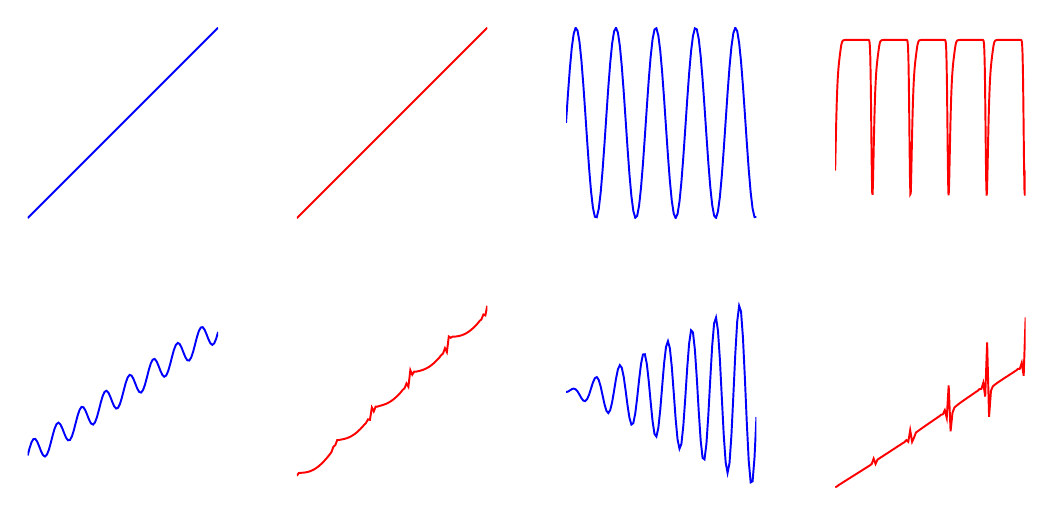
\begin{tikzpicture}

\begin{groupplot}[group style={group size=4 by 2}]
\nextgroupplot[
hide x axis,
hide y axis,
xmin=0, xmax=10,
ymin=0, ymax=20,
width=4cm,
height=4cm
]
\addplot [line width=0.7000000000000001pt, blue]
coordinates {
(1.77635683940025e-15,0)
(0.101010101010103,0.202020202020202)
(0.202020202020204,0.404040404040404)
(0.303030303030305,0.606060606060606)
(0.404040404040406,0.808080808080808)
(0.505050505050507,1.01010101010101)
(0.606060606060608,1.21212121212121)
(0.707070707070709,1.41414141414141)
(0.80808080808081,1.61616161616162)
(0.909090909090911,1.81818181818182)
(1.01010101010101,2.02020202020202)
(1.11111111111111,2.22222222222222)
(1.21212121212121,2.42424242424242)
(1.31313131313132,2.62626262626263)
(1.41414141414142,2.82828282828283)
(1.51515151515152,3.03030303030303)
(1.61616161616162,3.23232323232323)
(1.71717171717172,3.43434343434343)
(1.81818181818182,3.63636363636364)
(1.91919191919192,3.83838383838384)
(2.02020202020202,4.04040404040404)
(2.12121212121212,4.24242424242424)
(2.22222222222222,4.44444444444444)
(2.32323232323233,4.64646464646465)
(2.42424242424243,4.84848484848485)
(2.52525252525253,5.05050505050505)
(2.62626262626263,5.25252525252525)
(2.72727272727273,5.45454545454545)
(2.82828282828283,5.65656565656566)
(2.92929292929293,5.85858585858586)
(3.03030303030303,6.06060606060606)
(3.13131313131313,6.26262626262626)
(3.23232323232323,6.46464646464646)
(3.33333333333334,6.66666666666667)
(3.43434343434344,6.86868686868687)
(3.53535353535354,7.07070707070707)
(3.63636363636364,7.27272727272727)
(3.73737373737374,7.47474747474747)
(3.83838383838384,7.67676767676768)
(3.93939393939394,7.87878787878788)
(4.04040404040404,8.08080808080808)
(4.14141414141414,8.28282828282828)
(4.24242424242424,8.48484848484848)
(4.34343434343435,8.68686868686869)
(4.44444444444445,8.88888888888889)
(4.54545454545455,9.09090909090909)
(4.64646464646465,9.29292929292929)
(4.74747474747475,9.49494949494949)
(4.84848484848485,9.6969696969697)
(4.94949494949495,9.8989898989899)
(5.05050505050505,10.1010101010101)
(5.15151515151515,10.3030303030303)
(5.25252525252526,10.5050505050505)
(5.35353535353536,10.7070707070707)
(5.45454545454546,10.9090909090909)
(5.55555555555556,11.1111111111111)
(5.65656565656566,11.3131313131313)
(5.75757575757576,11.5151515151515)
(5.85858585858586,11.7171717171717)
(5.95959595959596,11.9191919191919)
(6.06060606060606,12.1212121212121)
(6.16161616161617,12.3232323232323)
(6.26262626262627,12.5252525252525)
(6.36363636363637,12.7272727272727)
(6.46464646464647,12.9292929292929)
(6.56565656565657,13.1313131313131)
(6.66666666666667,13.3333333333333)
(6.76767676767677,13.5353535353535)
(6.86868686868687,13.7373737373737)
(6.96969696969697,13.9393939393939)
(7.07070707070707,14.1414141414141)
(7.17171717171717,14.3434343434343)
(7.27272727272728,14.5454545454545)
(7.37373737373738,14.7474747474747)
(7.47474747474748,14.9494949494949)
(7.57575757575758,15.1515151515152)
(7.67676767676768,15.3535353535354)
(7.77777777777778,15.5555555555556)
(7.87878787878788,15.7575757575758)
(7.97979797979798,15.959595959596)
(8.08080808080808,16.1616161616162)
(8.18181818181819,16.3636363636364)
(8.28282828282829,16.5656565656566)
(8.38383838383839,16.7676767676768)
(8.48484848484849,16.969696969697)
(8.58585858585859,17.1717171717172)
(8.68686868686869,17.3737373737374)
(8.78787878787879,17.5757575757576)
(8.88888888888889,17.7777777777778)
(8.98989898989899,17.979797979798)
(9.09090909090909,18.1818181818182)
(9.1919191919192,18.3838383838384)
(9.2929292929293,18.5858585858586)
(9.3939393939394,18.7878787878788)
(9.4949494949495,18.989898989899)
(9.5959595959596,19.1919191919192)
(9.6969696969697,19.3939393939394)
(9.7979797979798,19.5959595959596)
(9.8989898989899,19.7979797979798)
(10,20)

};
\path [draw=white!15.0!black, fill opacity=0] (axis cs:13,20)--(axis cs:13,20);

\path [draw=white!15.0!black, fill opacity=0] (axis cs:10,13)--(axis cs:10,13);

\path [draw=white!15.0!black, fill opacity=0] (axis cs:13,0)--(axis cs:13,0);

\path [draw=white!15.0!black, fill opacity=0] (axis cs:1.77635683940025e-15,13)--(axis cs:1.77635683940025e-15,13);

\nextgroupplot[
hide x axis,
hide y axis,
xmin=0, xmax=10,
ymin=0, ymax=20,
width=4cm,
height=4cm
]
\addplot [line width=0.7000000000000001pt, red]
coordinates {
(0,0)
(0.101010101010101,0.202020202020202)
(0.202020202020202,0.404040404040404)
(0.303030303030303,0.606060606060606)
(0.404040404040404,0.808080808080808)
(0.505050505050505,1.01010101010101)
(0.606060606060606,1.21212121212121)
(0.707070707070707,1.41414141414141)
(0.808080808080808,1.61616161616162)
(0.909090909090909,1.81818181818182)
(1.01010101010101,2.02020202020202)
(1.11111111111111,2.22222222222222)
(1.21212121212121,2.42424242424242)
(1.31313131313131,2.62626262626263)
(1.41414141414141,2.82828282828283)
(1.51515151515152,3.03030303030303)
(1.61616161616162,3.23232323232323)
(1.71717171717172,3.43434343434343)
(1.81818181818182,3.63636363636364)
(1.91919191919192,3.83838383838384)
(2.02020202020202,4.04040404040404)
(2.12121212121212,4.24242424242424)
(2.22222222222222,4.44444444444444)
(2.32323232323232,4.64646464646465)
(2.42424242424242,4.84848484848485)
(2.52525252525253,5.05050505050505)
(2.62626262626263,5.25252525252525)
(2.72727272727273,5.45454545454545)
(2.82828282828283,5.65656565656566)
(2.92929292929293,5.85858585858586)
(3.03030303030303,6.06060606060606)
(3.13131313131313,6.26262626262626)
(3.23232323232323,6.46464646464646)
(3.33333333333333,6.66666666666667)
(3.43434343434344,6.86868686868687)
(3.53535353535354,7.07070707070707)
(3.63636363636364,7.27272727272727)
(3.73737373737374,7.47474747474747)
(3.83838383838384,7.67676767676768)
(3.93939393939394,7.87878787878788)
(4.04040404040404,8.08080808080808)
(4.14141414141414,8.28282828282828)
(4.24242424242424,8.48484848484848)
(4.34343434343434,8.68686868686869)
(4.44444444444445,8.88888888888889)
(4.54545454545455,9.09090909090909)
(4.64646464646465,9.29292929292929)
(4.74747474747475,9.49494949494949)
(4.84848484848485,9.6969696969697)
(4.94949494949495,9.8989898989899)
(5.05050505050505,10.1010101010101)
(5.15151515151515,10.3030303030303)
(5.25252525252525,10.5050505050505)
(5.35353535353535,10.7070707070707)
(5.45454545454546,10.9090909090909)
(5.55555555555556,11.1111111111111)
(5.65656565656566,11.3131313131313)
(5.75757575757576,11.5151515151515)
(5.85858585858586,11.7171717171717)
(5.95959595959596,11.9191919191919)
(6.06060606060606,12.1212121212121)
(6.16161616161616,12.3232323232323)
(6.26262626262626,12.5252525252525)
(6.36363636363637,12.7272727272727)
(6.46464646464647,12.9292929292929)
(6.56565656565657,13.1313131313131)
(6.66666666666667,13.3333333333333)
(6.76767676767677,13.5353535353535)
(6.86868686868687,13.7373737373737)
(6.96969696969697,13.9393939393939)
(7.07070707070707,14.1414141414141)
(7.17171717171717,14.3434343434343)
(7.27272727272727,14.5454545454545)
(7.37373737373738,14.7474747474747)
(7.47474747474748,14.9494949494949)
(7.57575757575758,15.1515151515152)
(7.67676767676768,15.3535353535354)
(7.77777777777778,15.5555555555556)
(7.87878787878788,15.7575757575758)
(7.97979797979798,15.959595959596)
(8.08080808080808,16.1616161616162)
(8.18181818181818,16.3636363636364)
(8.28282828282828,16.5656565656566)
(8.38383838383839,16.7676767676768)
(8.48484848484849,16.969696969697)
(8.58585858585859,17.1717171717172)
(8.68686868686869,17.3737373737374)
(8.78787878787879,17.5757575757576)
(8.88888888888889,17.7777777777778)
(8.98989898989899,17.979797979798)
(9.09090909090909,18.1818181818182)
(9.19191919191919,18.3838383838384)
(9.29292929292929,18.5858585858586)
(9.3939393939394,18.7878787878788)
(9.4949494949495,18.989898989899)
(9.5959595959596,19.1919191919192)
(9.6969696969697,19.3939393939394)
(9.7979797979798,19.5959595959596)
(9.8989898989899,19.7979797979798)
(10,20)

};
\path [draw=white!15.0!black, fill opacity=0] (axis cs:13,20)--(axis cs:13,20);

\path [draw=white!15.0!black, fill opacity=0] (axis cs:10,13)--(axis cs:10,13);

\path [draw=white!15.0!black, fill opacity=0] (axis cs:13,0)--(axis cs:13,0);

\path [draw=white!15.0!black, fill opacity=0] (axis cs:0,13)--(axis cs:0,13);

\nextgroupplot[
hide x axis,
hide y axis,
xmin=0, xmax=10,
ymin=-1, ymax=1,
width=4cm,
height=4cm
]
\addplot [line width=0.7000000000000001pt, blue]
coordinates {
(3.5527136788005e-15,0)
(0.101010101010105,0.298413804447641)
(0.202020202020206,0.569634106908966)
(0.303030303030307,0.788945462844257)
(0.404040404040408,0.936362725104285)
(0.505050505050509,0.998452226900389)
(0.60606060606061,0.969555949182324)
(0.707070707070711,0.852307117939675)
(0.808080808080812,0.657390246682775)
(0.909090909090913,0.402567490669497)
(1.01010101010101,0.11106003812413)
(1.11111111111111,-0.190567962875485)
(1.21212121212122,-0.47483011082224)
(1.31313131313132,-0.71582249922919)
(1.41414141414142,-0.89158425733514)
(1.51515151515152,-0.98609877449093)
(1.61616161616162,-0.990753243005677)
(1.71717171717172,-0.905123515950137)
(1.81818181818182,-0.737012758318913)
(1.91919191919192,-0.501740369393911)
(2.02020202020202,-0.220745974555063)
(2.12121212121213,0.0803642996702817)
(2.22222222222223,0.37415123057122)
(2.32323232323233,0.633842948448905)
(2.42424242424243,0.835774572052259)
(2.52525252525253,0.961544714026824)
(2.62626262626263,0.999692340886112)
(2.72727272727273,0.946741180583354)
(2.82828282828283,0.807516504139563)
(2.92929292929293,0.594705414024498)
(3.03030303030303,0.3277007088135)
(3.13131313131314,0.0308336790611428)
(3.23232323232324,-0.268843125910384)
(3.33333333333334,-0.54402111088937)
(3.43434343434344,-0.769624180301191)
(3.53535353535354,-0.925093843135269)
(3.63636363636364,-0.996262642919822)
(3.73737373737374,-0.976645193022395)
(3.83838383838384,-0.868029169330635)
(3.93939393939394,-0.680312405027813)
(4.04040404040405,-0.430600932498663)
(4.14141414141415,-0.141650164941304)
(4.24242424242425,0.160208732147209)
(4.34343434343435,0.447468316432701)
(4.44444444444445,0.693951534577056)
(4.54545454545455,0.877197153948597)
(4.64646464646465,0.980506583396065)
(4.74747474747475,0.994465562811467)
(4.84848484848485,0.917802054746127)
(4.94949494949495,0.757502161142318)
(5.05050505050505,0.528173502056996)
(5.15151515151516,0.25071406965208)
(5.25252525252526,-0.0495921394416738)
(5.35353535353536,-0.345379174414414)
(5.45454545454546,-0.609692902437243)
(5.55555555555556,-0.818447253157943)
(5.65656565656566,-0.952619105774571)
(5.75757575757576,-0.999981805600717)
(5.85858585858586,-0.956219340264959)
(5.95959595959596,-0.825319644206981)
(6.06060606060607,-0.61921119088112)
(6.16161616161617,-0.356675988865319)
(6.26262626262627,-0.0616380370868764)
(6.36363636363637,0.239016793197097)
(6.46464646464647,0.517890782435197)
(6.56565656565657,0.749571029926278)
(6.66666666666667,0.912945250727628)
(6.76767676767677,0.993125671111422)
(6.86868686868687,0.982805704088478)
(6.96969696969698,0.882925775468708)
(7.07070707070708,0.702587625844653)
(7.17171717171718,0.458224897886049)
(7.27272727272728,0.172105590690409)
(7.37373737373738,-0.129697152232876)
(7.47474747474748,-0.419681005700317)
(7.57575757575758,-0.671420662377814)
(7.67676767676768,-0.861975887089034)
(7.77777777777778,-0.973981987569556)
(7.87878787878788,-0.997232203708085)
(7.97979797979798,-0.92960781717014)
(8.08080808080809,-0.777271223469046)
(8.18181818181819,-0.554104372439755)
(8.28282828282829,-0.280443750251132)
(8.38383838383839,0.0187728199728824)
(8.48484848484849,0.316278682751012)
(8.58585858585859,0.584963073936907)
(8.68686868686869,0.800341638529193)
(8.78787878787879,0.942787612159873)
(8.88888888888889,0.999320345780098)
(8.98989898989899,0.964788190970519)
(9.0909090909091,0.842337953295793)
(9.1919191919192,0.643128133910366)
(9.2929292929293,0.385312090797061)
(9.3939393939394,0.0923837809243858)
(9.4949494949495,-0.208963169415405)
(9.5959595959596,-0.491267969968986)
(9.6969696969697,-0.728805081099179)
(9.7979797979798,-0.899928500486141)
(9.89898989898991,-0.989044294552925)
(10,-0.988031624092862)

};
\path [draw=white!15.0!black, fill opacity=0] (axis cs:13,1)--(axis cs:13,1);

\path [draw=white!15.0!black, fill opacity=0] (axis cs:10,13)--(axis cs:10,13);

\path [draw=white!15.0!black, fill opacity=0] (axis cs:13,-1)--(axis cs:13,-1);

\path [draw=white!15.0!black, fill opacity=0] (axis cs:3.5527136788005e-15,13)--(axis cs:3.5527136788005e-15,13);

\nextgroupplot[
hide x axis,
hide y axis,
xmin=0, xmax=10,
ymin=1, ymax=9,
width=4cm,
height=4cm
]
\addplot [line width=0.7000000000000001pt, red]
coordinates {
(0,3.0000000015)
(0.0200400801603206,3.77633368354401)
(0.0400801603206413,4.52460123431942)
(0.0601202404809619,5.19976564438721)
(0.0801603206412826,5.77665698346634)
(0.100200400801603,6.25013774664831)
(0.120240480961924,6.62949731389832)
(0.140280561122244,6.93103782944216)
(0.160320641282565,7.1721211130598)
(0.180360721442886,7.36806079284994)
(0.200400801603206,7.53164904109355)
(0.220440881763527,7.67409096509046)
(0.240480961923848,7.80531368144426)
(0.260521042084168,7.93210937904091)
(0.280561122244489,8.05530176731567)
(0.30060120240481,8.16941963896676)
(0.32064128256513,8.2665039261016)
(0.340681362725451,8.34131044574021)
(0.360721442885772,8.39383225561936)
(0.380761523046092,8.42811201219364)
(0.400801603206413,8.44950217644931)
(0.420841683366733,8.46265441583477)
(0.440881763527054,8.47083577810201)
(0.460921843687375,8.47606636245024)
(0.480961923847695,8.47951194151019)
(0.501002004008016,8.48183810846979)
(0.521042084168337,8.48343724532027)
(0.541082164328657,8.48454981991136)
(0.561122244488978,8.48532920125263)
(0.581162324649299,8.48587769113936)
(0.601202404809619,8.48626513759441)
(0.62124248496994,8.48653938165659)
(0.64128256513026,8.48673368476291)
(0.661322645290581,8.48687154795143)
(0.681362725450902,8.48696948212261)
(0.701402805611222,8.48703906009843)
(0.721442885771543,8.48708851428477)
(0.741482965931864,8.48712370450462)
(0.761523046092184,8.48714874898051)
(0.781563126252505,8.48716656159826)
(0.801603206412826,8.48717923185596)
(0.821643286573146,8.48718824753238)
(0.841683366733467,8.48719466214212)
(0.861723446893788,8.48719922820505)
(0.881763527054108,8.48720248035432)
(0.901803607214429,8.48720479362567)
(0.921843687374749,8.48720643549146)
(0.94188376753507,8.48720760147584)
(0.961923847695391,8.48720843290083)
(0.981963927855711,8.4872090286148)
(1.00200400801603,8.48720945604496)
(1.02204408817635,8.48720976099459)
(1.04208416833667,8.48720997619621)
(1.06212424849699,8.48721012710931)
(1.08216432865731,8.48721023327678)
(1.10220440881764,8.48721030774573)
(1.12224448897796,8.48721035846094)
(1.14228456913828,8.48721039152709)
(1.1623246492986,8.48721041323478)
(1.18236472945892,8.4872104294582)
(1.20240480961924,8.48721044403844)
(1.22244488977956,8.48721045822997)
(1.24248496993988,8.48721047154691)
(1.2625250501002,8.48721048296447)
(1.28256513026052,8.48721049167154)
(1.30260521042084,8.48721049744502)
(1.32264529058116,8.48721050082309)
(1.34268537074148,8.48721050280605)
(1.3627254509018,8.48721050404016)
(1.38276553106212,8.48721050427593)
(1.40280561122244,8.48721050284608)
(1.42284569138277,8.48721049967624)
(1.44288577154309,8.48721049564682)
(1.46292585170341,8.48721049199211)
(1.48296593186373,8.48721048953661)
(1.50300601202405,8.487210488503)
(1.52304609218437,8.48721048883474)
(1.54308617234469,8.48721049056553)
(1.56312625250501,8.48721049406479)
(1.58316633266533,8.48721050121259)
(1.60320641282565,8.48721052212866)
(1.62324649298597,8.48721060390191)
(1.64328657314629,8.48721093738651)
(1.66332665330661,8.48721217831945)
(1.68336673346693,8.48721576801692)
(1.70340681362725,8.48721828303868)
(1.72344689378758,8.48715070295623)
(1.7434869739479,8.48649310890813)
(1.76352705410822,8.48252213601719)
(1.78356713426854,8.46448870084599)
(1.80360721442886,8.39992375288832)
(1.82364729458918,8.21430132121412)
(1.8436873747495,7.78222353454685)
(1.86372745490982,6.9668553418325)
(1.88376753507014,5.72773931231706)
(1.90380761523046,4.23982947223482)
(1.92384769539078,2.89081042453935)
(1.9438877755511,2.08400291751364)
(1.96392785571142,1.98124620843053)
(1.98396793587174,2.43288082149205)
(2.00400801603206,3.15373096329888)
(2.02404809619238,3.93026811640625)
(2.04408817635271,4.66672800470541)
(2.06412825651303,5.3234973896961)
(2.08416833667335,5.87971022130918)
(2.10420841683367,6.33314577450474)
(2.12424849699399,6.69561556122598)
(2.14428857715431,6.98371252413022)
(2.16432865731463,7.21458282047253)
(2.18436873747495,7.40314785142412)
(2.20440881763527,7.56161987148983)
(2.22444889779559,7.70107357587123)
(2.24448897795591,7.83104897058474)
(2.26452905811623,7.95726062319658)
(2.28456913827655,8.07923673762562)
(2.30460921843687,8.19057617511737)
(2.32464929859719,8.2834527081577)
(2.34468937875751,8.35364510168904)
(2.36472945891784,8.40211573557939)
(2.38476953907816,8.4333842754026)
(2.40480961923848,8.45280289564775)
(2.4248496993988,8.4647429546596)
(2.44488977955912,8.47220276654406)
(2.46492985971944,8.47700770264392)
(2.48496993987976,8.48018502317643)
(2.50501002004008,8.48233993404139)
(2.5250501002004,8.48382827592742)
(2.54509018036072,8.48486198341539)
(2.56513026052104,8.48558870516879)
(2.58517034068136,8.48610113252678)
(2.60521042084168,8.48646137745015)
(2.625250501002,8.48671805702338)
(2.64529058116232,8.48689960759109)
(2.66533066132265,8.48702766876231)
(2.68537074148297,8.48711973715459)
(2.70541082164329,8.48718456406307)
(2.72545090180361,8.48723049251931)
(2.74549098196393,8.48726376228567)
(2.76553106212425,8.48728693474266)
(2.78557114228457,8.48730352980816)
(2.80561122244489,8.48731557084587)
(2.82565130260521,8.48732380864855)
(2.84569138276553,8.48732985002716)
(2.86573146292585,8.48733419584296)
(2.88577154308617,8.48733711659743)
(2.90581162324649,8.48733934446329)
(2.92585170340681,8.48734089000268)
(2.94589178356713,8.48734191887079)
(2.96593186372745,8.48734274984855)
(2.98597194388778,8.48734329454423)
(3.0060120240481,8.48734367073866)
(3.02605210420842,8.48734398668873)
(3.04609218436874,8.4873441729695)
(3.06613226452906,8.48734430683964)
(3.08617234468938,8.487344419898)
(3.1062124248497,8.48734448355128)
(3.12625250501002,8.48734452400993)
(3.14629258517034,8.48734456137317)
(3.16633266533066,8.48734458650182)
(3.18637274549098,8.48734458484421)
(3.2064128256513,8.48734461297743)
(3.22645290581162,8.4873446361062)
(3.24649298597194,8.48734461471638)
(3.26653306613226,8.48734466270723)
(3.28657314629258,8.48734466714856)
(3.30661322645291,8.48734462389993)
(3.32665330661323,8.48734470396229)
(3.34669338677355,8.48734466116082)
(3.36673346693387,8.48734461850023)
(3.38677354709419,8.48734474651204)
(3.40681362725451,8.48734461660312)
(3.42685370741483,8.48734462212139)
(3.44689378757515,8.48734478526844)
(3.46693386773547,8.48734452126267)
(3.48697394789579,8.48734467052548)
(3.50701402805611,8.4873448118048)
(3.52705410821643,8.48734438900019)
(3.54709418837675,8.48734481906501)
(3.56713426853707,8.48734478357614)
(3.58717434869739,8.48734424877728)
(3.60721442885772,8.48734513708857)
(3.62725450901804,8.48734473287117)
(3.64729458917836,8.48734471942384)
(3.66733466933868,8.48734768989865)
(3.687374749499,8.48735040878775)
(3.70741482965932,8.48734954417312)
(3.72745490981964,8.48723763253716)
(3.74749498997996,8.48626624627782)
(3.76753507014028,8.48078203784181)
(3.7875751503006,8.45708203712698)
(3.80761523046092,8.37594659169322)
(3.82765531062124,8.15244396581692)
(3.84769539078156,7.65350425272208)
(3.86773547094188,6.75110455030618)
(3.8877755511022,5.44015641200143)
(3.90781563126252,3.9445720059844)
(3.92785571142285,2.67625331937318)
(3.94789579158317,2.00813101960839)
(3.96793587174349,2.03614117492511)
(3.98797595190381,2.56430337701983)
(4.00801603206413,3.30909710800474)
(4.02805611222445,4.08247245974705)
(4.04809619238477,4.80540588466389)
(4.06813627254509,5.44318661538898)
(4.08817635270541,5.97842185728842)
(4.10821643286573,6.41246536055823)
(4.12825651302605,6.75867494768912)
(4.14829659318637,7.0339895097997)
(4.16833667334669,7.25530995144829)
(4.18837675350701,7.43693417170416)
(4.20841683366733,7.59074229885283)
(4.22845691382765,7.72762096230826)
(4.24849699398798,7.85655631976342)
(4.2685370741483,7.98218100803522)
(4.28857715430862,8.10267278402982)
(4.30861723446894,8.2108869152034)
(4.32865731462926,8.29939552841505)
(4.34869739478958,8.36501547905053)
(4.3687374749499,8.40961917067907)
(4.38877755511022,8.43810530074993)
(4.40881763527054,8.45572318755974)
(4.42885771543086,8.46656908285041)
(4.44889779559118,8.47338371345891)
(4.4689378757515,8.47779871361709)
(4.48897795591182,8.48073252977445)
(4.50901803607214,8.48273191964218)
(4.52905811623246,8.48411501582931)
(4.54909819639279,8.48507727275651)
(4.56913827655311,8.48575525398829)
(4.58917835671343,8.48623265669693)
(4.60921843687375,8.48656893346536)
(4.62925851703407,8.48680879742)
(4.64929859719439,8.48697791705785)
(4.66933867735471,8.48709770189203)
(4.68937875751503,8.48718375285581)
(4.70941883767535,8.48724409117617)
(4.72945891783567,8.48728716826046)
(4.74949899799599,8.48731821800454)
(4.76953907815631,8.48733977654567)
(4.78957915831663,8.4873553937631)
(4.80961923847695,8.48736658345782)
(4.82965931863727,8.48737425940778)
(4.8496993987976,8.48737996614599)
(4.86973947895792,8.48738397523161)
(4.88977955911824,8.487386712775)
(4.90981963927856,8.48738881992133)
(4.92985971943888,8.48739022818392)
(4.9498997995992,8.48739120786494)
(4.96993987975952,8.48739199140779)
(4.98997995991984,8.48739248197404)
(5.01002004008016,8.48739284819026)
(5.03006012024048,8.4873931419659)
(5.0501002004008,8.48739330722788)
(5.07014028056112,8.48739343964675)
(5.09018036072144,8.48739354373619)
(5.11022044088176,8.48739359797412)
(5.13026052104208,8.48739363921171)
(5.1503006012024,8.48739367443326)
(5.17034068136272,8.48739369348747)
(5.19038076152305,8.48739369542262)
(5.21042084168337,8.48739372736577)
(5.23046092184369,8.48739373857513)
(5.25050100200401,8.48739372729401)
(5.27054108216433,8.48739377723582)
(5.29058116232465,8.48739376259272)
(5.31062124248497,8.48739374171663)
(5.33066132264529,8.48739381426647)
(5.35070140280561,8.48739374998099)
(5.37074148296593,8.48739374736177)
(5.39078156312625,8.48739384655452)
(5.41082164328657,8.48739370195702)
(5.43086172344689,8.48739376849633)
(5.45090180360721,8.48739386234515)
(5.47094188376753,8.48739361449494)
(5.49098196392786,8.48739383698676)
(5.51102204408818,8.48739385053586)
(5.5310621242485,8.48739351229872)
(5.55110220440882,8.48739399789198)
(5.57114228456914,8.48739376626818)
(5.59118236472946,8.48739344128578)
(5.61122244488978,8.48739431027347)
(5.6312625250501,8.4873936915794)
(5.65130260521042,8.48739421562926)
(5.67134268537074,8.48739735968866)
(5.69138276553106,8.4874002826689)
(5.71142284569138,8.48739347389445)
(5.7314629258517,8.48721112003616)
(5.75150300601202,8.48580308524609)
(5.77154308617234,8.47830689778545)
(5.79158316633267,8.44744303261206)
(5.81162324649299,8.34637115305202)
(5.83166332665331,8.07950143857955)
(5.85170340681363,7.50816684141747)
(5.87174348697395,6.51812991356001)
(5.89178356713427,5.14440083519052)
(5.91182364729459,3.65843098947308)
(5.93186372745491,2.48662943263326)
(5.95190380761523,1.96105831149268)
(5.97194388777555,2.11121597672057)
(5.99198396793587,2.7039478346136)
(6.01202404809619,3.46520596527384)
(6.03206412825651,4.23253152007943)
(6.05210420841683,4.94061644990345)
(6.07214428857715,5.55868860554133)
(6.09218436873747,6.07303147398607)
(6.1122244488978,6.48824550751378)
(6.13226452905812,6.81888131544828)
(6.15230460921844,7.08209991349325)
(6.17234468937876,7.29444035045902)
(6.19238476953908,7.46959273984324)
(6.2124248496994,7.61917597778321)
(6.23246492985972,7.75384739345756)
(6.25250501002004,7.88193653640828)
(6.27254509018036,8.00689818861089)
(6.29258517034068,8.12560120631247)
(6.312625250501,8.23037696884967)
(6.33266533066132,8.31438828014212)
(6.35270541082164,8.37551827432363)
(6.37274549098196,8.41646042595415)
(6.39278557114228,8.44237884928672)
(6.4128256513026,8.45836006179391)
(6.43286573146293,8.46822055373079)
(6.45290581162325,8.47445389775742)
(6.47294589178357,8.47851454895827)
(6.49298597194389,8.48122636763792)
(6.51302605210421,8.48308260111039)
(6.53306613226453,8.48436806038857)
(6.55310621242485,8.4852643521995)
(6.57314629258517,8.48589682520669)
(6.59318637274549,8.48634155405377)
(6.61322645290581,8.48665568156779)
(6.63326653306613,8.48687969227162)
(6.65330661322645,8.48703724826537)
(6.67334669338677,8.48714939520121)
(6.69338677354709,8.48722971166118)
(6.71342685370741,8.48728591968835)
(6.73346693386774,8.48732634985109)
(6.75350701402806,8.48735526327667)
(6.77354709418838,8.48737536680438)
(6.7935871743487,8.48739006190309)
(6.81362725450902,8.48740042840574)
(6.83366733466934,8.4874076148801)
(6.85370741482966,8.48741299268396)
(6.87374749498998,8.48741667906288)
(6.8937875751503,8.48741926766268)
(6.91382765531062,8.48742124510094)
(6.93386773547094,8.48742252959202)
(6.95390781563126,8.48742346722773)
(6.97394789579158,8.48742419590678)
(6.9939879759519,8.48742464256753)
(7.01402805611222,8.48742500236366)
(7.03406813627254,8.48742526804462)
(7.05410821643287,8.48742541789121)
(7.07414829659319,8.48742555157548)
(7.09418837675351,8.48742564288521)
(7.11422845691383,8.48742569169218)
(7.13426853707415,8.48742573275752)
(7.15430861723447,8.4874257678009)
(7.17434869739479,8.48742577758389)
(7.19438877755511,8.4874257848198)
(7.21442885771543,8.4874258188624)
(7.23446893787575,8.48742581998343)
(7.25450901803607,8.48742581995971)
(7.27454909819639,8.48742586790839)
(7.29458917835671,8.4874258379235)
(7.31462925851703,8.48742584104512)
(7.33466933867735,8.48742589815753)
(7.35470941883768,8.48742581848689)
(7.374749498998,8.48742586216494)
(7.39478957915832,8.48742591488721)
(7.41482965931864,8.48742577157056)
(7.43486973947896,8.48742589646191)
(7.45490981963928,8.48742590438143)
(7.4749498997996,8.4874257014825)
(7.49498997995992,8.48742597947842)
(7.51503006012024,8.48742585034231)
(7.53507014028056,8.48742564540607)
(7.55511022044088,8.48742613639122)
(7.5751503006012,8.48742570883431)
(7.59519038076152,8.48742566988393)
(7.61523046092184,8.48742641095919)
(7.63527054108216,8.48742564318922)
(7.65531062124249,8.48742682080218)
(7.67535070140281,8.4874300186428)
(7.69539078156313,8.48743299664418)
(7.71543086172345,8.48741547111654)
(7.73547094188377,8.48712844629946)
(7.75551102204409,8.48511482319364)
(7.77555110220441,8.47497230052991)
(7.79559118236473,8.43514379761245)
(7.81563126252505,8.31031320125501)
(7.83567134268537,7.99431717047088)
(7.85571142284569,7.34557507169895)
(7.87575150300601,6.26895279311564)
(7.89579158316633,4.8435535522876)
(7.91583166332665,3.38515667028407)
(7.93587174348697,2.32393572467939)
(7.95591182364729,1.9419328568076)
(7.97595190380761,2.20406009222128)
(7.99599198396794,2.84987131116013)
(8.01603206412826,3.62122317661332)
(8.03607214428858,4.38013383857603)
(8.0561122244489,5.07216899478219)
(8.07615230460922,5.66996668450781)
(8.09619238476954,6.16363840720038)
(8.11623246492986,6.56062780403204)
(8.13627254509018,6.87638452949362)
(8.1563126252505,7.1281781718944)
(8.17635270541082,7.33208163511714)
(8.19639278557114,7.50122206170809)
(8.21643286573146,7.64701201512097)
(8.23647294589178,7.77981808118255)
(8.2565130260521,7.90720647310492)
(8.27655310621243,8.03137318991964)
(8.29659318637274,8.14796077781657)
(8.31663326653307,8.24901127151345)
(8.33667334669339,8.32844114472396)
(8.35671342685371,8.38519742711796)
(8.37675350701403,8.4226935392777)
(8.39679358717435,8.446251301801)
(8.41683366733467,8.46074823116716)
(8.43687374749499,8.46972215862385)
(8.45691382765531,8.47543094913838)
(8.47695390781563,8.47916920952149)
(8.49699398797595,8.48167848863257)
(8.51703406813627,8.48340257231624)
(8.53707414829659,8.48459751805932)
(8.55711422845691,8.48543288410679)
(8.57715430861723,8.48602274532875)
(8.59719438877755,8.48643710315581)
(8.61723446893788,8.48673071603464)
(8.6372745490982,8.48693974103363)
(8.65731462925852,8.48708661535763)
(8.67735470941884,8.4871916576824)
(8.69739478957916,8.48726651337386)
(8.71743486973948,8.48731895631905)
(8.7374749498998,8.48735689798615)
(8.75751503006012,8.48738377041015)
(8.77755511022044,8.48740257620175)
(8.79759519038076,8.48741637422965)
(8.81763527054108,8.48742596516603)
(8.8376753507014,8.48743272694452)
(8.85771543086172,8.48743776792982)
(8.87775551102204,8.48744116062307)
(8.89779559118236,8.48744362034202)
(8.91783567134268,8.48744545946732)
(8.93787575150301,8.48744663805123)
(8.95791583166333,8.48744754358458)
(8.97795591182365,8.48744821000763)
(8.99799599198397,8.48744862330551)
(9.01803607214429,8.48744897323819)
(9.03807615230461,8.4874492119536)
(9.05811623246493,8.48744935250615)
(9.07815631262525,8.48744948100806)
(9.09819639278557,8.48744956175571)
(9.11823647294589,8.48744960602693)
(9.13827655310621,8.48744964702526)
(9.15831663326653,8.48744967868322)
(9.17835671342685,8.48744968317053)
(9.19839679358717,8.48744969712033)
(9.21843687374749,8.48744973133109)
(9.23847695390782,8.48744972065323)
(9.25851703406814,8.48744973650387)
(9.27855711422846,8.48744977532504)
(9.29859719438878,8.48744973502839)
(9.3186372745491,8.48744976366688)
(9.33867735470942,8.48744979572656)
(9.35871743486974,8.48744971684561)
(9.37875751503006,8.48744979490311)
(9.39879759519038,8.48744979571433)
(9.4188376753507,8.48744967684038)
(9.43887775551102,8.48744983903781)
(9.45891783567134,8.48744975599252)
(9.47895791583166,8.487449635745)
(9.49899799599198,8.48744992231563)
(9.5190380761523,8.48744966552392)
(9.53907815631263,8.48744963605416)
(9.55911823647295,8.48745004908807)
(9.57915831663327,8.48744949118328)
(9.59919839679359,8.48744975826813)
(9.61923847695391,8.48745025433437)
(9.63927855711423,8.48744950176366)
(9.65931863727455,8.48745133757689)
(9.67935871743487,8.48745449789585)
(9.69939879759519,8.4874571864995)
(9.71943887775551,8.48742138823657)
(9.73947895791583,8.48698161092845)
(9.75951903807615,8.48413737868168)
(9.77955911823647,8.47054905488806)
(9.79959919839679,8.41961185428491)
(9.81963927855711,8.2667455390477)
(9.83967935871743,7.89569364872449)
(9.85971943887776,7.16527696440282)
(9.87975951903808,6.00496808409882)
(9.8997995991984,4.54093541463698)
(9.91983967935872,3.12827882687689)
(9.93987975951904,2.18955441843019)
(9.95991983967936,1.94935414755582)
(9.97995991983968,2.31216833553208)
(10,3.0003435289271)

};
\path [draw=white!15.0!black, fill opacity=0] (axis cs:13,9)--(axis cs:13,9);

\path [draw=white!15.0!black, fill opacity=0] (axis cs:10,13)--(axis cs:10,13);

\path [draw=white!15.0!black, fill opacity=0] (axis cs:13,1)--(axis cs:13,1);

\path [draw=white!15.0!black, fill opacity=0] (axis cs:0,13)--(axis cs:0,13);

\nextgroupplot[
hide x axis,
hide y axis,
xmin=0, xmax=10,
ymin=-5, ymax=25,
width=4cm,
height=4cm
]
\addplot [line width=0.7000000000000001pt, blue]
coordinates {
(1.77635683940025e-15,0)
(0.101010101010103,1.16972348289607)
(0.202020202020204,2.09781153124637)
(0.303030303030305,2.60296505986138)
(0.404040404040406,2.60949170048672)
(0.505050505050507,2.16620618031416)
(0.606060606060608,1.43424128836947)
(0.707070707070709,0.646813030529189)
(0.80808080808081,0.0509866108532118)
(0.909090909090911,-0.154015730800041)
(1.01010101010101,0.133439503310022)
(1.11111111111111,0.892019192264577)
(1.21212121212121,1.9827504751323)
(1.31313131313132,3.18372226361774)
(1.41414141414142,4.24549642368126)
(1.51515151515152,4.95339245835668)
(1.61616161616162,5.1810932112743)
(1.71717171717172,4.92218625085713)
(1.81818181818182,4.29176505399064)
(1.91919191919192,3.49769017372765)
(2.02020202020202,2.78868647523401)
(2.12121212121212,2.3922365561537)
(2.22222222222222,2.45777835953462)
(2.32323232323233,3.01939053098336)
(2.42424242424243,3.98728298348752)
(2.52525252525253,5.17021747521253)
(2.62626262626263,6.32325978372769)
(2.72727272727273,7.20893976244265)
(2.82828282828283,7.65654761788272)
(2.92929292929293,7.60476013194383)
(3.03030303030303,7.11695306472005)
(3.13131313131313,6.36537623209961)
(3.23232323232323,5.58814274003209)
(3.33333333333334,5.02977216035078)
(3.43434343434344,4.88013401255833)
(3.53535353535354,5.22703735946139)
(3.63636363636364,6.03430489096503)
(3.73737373737374,7.15080639561124)
(3.83838383838384,8.34819596271544)
(3.93939393939394,9.37792993864043)
(4.04040404040404,10.0333282579265)
(4.14141414141414,10.2011824396848)
(4.24242424242424,9.89002373653779)
(4.34343434343435,9.22799288149768)
(4.44444444444445,8.43084335682357)
(4.54545454545455,7.74806776615346)
(4.64646464646465,7.40059955063213)
(4.74747474747475,7.52564592570927)
(4.84848484848485,8.14242725003161)
(4.94949494949495,9.14737770337224)
(5.05050505050505,10.3400056639479)
(5.15151515151515,11.4729564509041)
(5.25252525252526,12.313776769033)
(5.35353535353536,12.702958278646)
(5.45454545454546,12.5937668156825)
(5.55555555555556,12.0639119088691)
(5.65656565656566,11.2961427163943)
(5.75757575757576,10.5326155752135)
(5.85858585858586,10.0144275824015)
(5.95959595959596,9.92141466862103)
(6.06060606060606,10.3272465801163)
(6.16161616161617,11.1810315487621)
(6.26262626262627,12.3200239626361)
(6.36363636363637,13.5102619327555)
(6.46464646464647,14.5049875586983)
(6.56565656565657,15.1062623572933)
(6.66666666666667,15.2143924865909)
(6.76767676767677,14.8528222905033)
(6.86868686868687,14.1622802479392)
(6.96969696969697,13.3656390824819)
(7.07070707070707,12.7122644605122)
(7.17171717171717,12.4157484035596)
(7.27272727272728,12.6005753770117)
(7.37373737373738,13.2710385287151)
(7.47474747474748,14.3101676902889)
(7.57575757575758,15.5089368191422)
(7.67676767676768,16.6184577851754)
(7.77777777777778,17.4121277176568)
(7.87878787878788,17.7422117245549)
(7.97979797979798,17.5767322836758)
(8.08080808080808,17.0074540274871)
(8.18181818181819,16.2269701214737)
(8.28282828282829,15.4806117655801)
(8.38383838383839,15.0051890125201)
(8.48484848484849,14.969859315891)
(8.58585858585859,15.4338889270665)
(8.68686868686869,16.3318541168028)
(8.78787878787879,17.4899774753814)
(8.88888888888889,18.6695201184033)
(8.98989898989899,19.6263947677971)
(9.09090909090909,20.1721143263146)
(9.1919191919192,20.2208570911657)
(9.2929292929293,19.8108964265813)
(9.3939393939394,19.0950439077188)
(9.4949494949495,18.3024922821398)
(9.5959595959596,17.6815860584331)
(9.6969696969697,17.4378099015879)
(9.7979797979798,17.6824791280055)
(9.8989898989899,18.4049442795857)
(10,19.4752502925921)

};
\path [draw=white!15.0!black, fill opacity=0] (axis cs:13,25)--(axis cs:13,25);

\path [draw=white!15.0!black, fill opacity=0] (axis cs:10,13)--(axis cs:10,13);

\path [draw=white!15.0!black, fill opacity=0] (axis cs:13,-5)--(axis cs:13,-5);

\path [draw=white!15.0!black, fill opacity=0] (axis cs:1.77635683940025e-15,13)--(axis cs:1.77635683940025e-15,13);

\nextgroupplot[
hide x axis,
hide y axis,
xmin=0, xmax=10,
ymin=0, ymax=50,
width=4cm,
height=4cm
]
\addplot [line width=0.7000000000000001pt, red]
coordinates {
(0,3.00000001818333)
(0.101010101010101,3.7365971690399)
(0.202020202020202,3.79087654972704)
(0.303030303030303,3.81972464802676)
(0.404040404040404,3.86984264141422)
(0.505050505050505,3.95108549475632)
(0.606060606060606,4.07026127425514)
(0.707070707070707,4.23311731435105)
(0.808080808080808,4.44410221745296)
(0.909090909090909,4.70622123954827)
(1.01010101010101,5.02093139416861)
(1.11111111111111,5.38818124893881)
(1.21212121212121,5.80656416272165)
(1.31313131313131,6.27356433024775)
(1.41414141414141,6.78585161264162)
(1.51515151515152,7.33958321248437)
(1.61616161616162,7.93067773052623)
(1.71717171717172,8.55526883914277)
(1.81818181818182,9.25305710242751)
(1.91919191919192,10.6353948171778)
(2.02020202020202,11.0647323455881)
(2.12121212121212,12.4079296240676)
(2.22222222222222,12.4074483200248)
(2.32323232323232,12.5299124420119)
(2.42424242424242,12.6174878857956)
(2.52525252525253,12.7404432981875)
(2.62626262626263,12.8935248555319)
(2.72727272727273,13.0882635968089)
(2.82828282828283,13.3286316001858)
(2.92929292929293,13.6183477947296)
(3.03030303030303,13.9588702689583)
(3.13131313131313,14.3504106893964)
(3.23232323232323,14.7908640252408)
(3.33333333333333,15.2802937470737)
(3.43434343434344,15.8059892465043)
(3.53535353535354,16.3984372960339)
(3.63636363636364,16.9289932614298)
(3.73737373737374,17.838703752751)
(3.83838383838384,17.7076390723261)
(3.93939393939394,20.9329946109412)
(4.04040404040404,19.920545917454)
(4.14141414141414,21.1930025321941)
(4.24242424242424,21.1962332892127)
(4.34343434343434,21.3689235464812)
(4.44444444444445,21.492363088748)
(4.54545454545455,21.6495025886986)
(4.64646464646465,21.8320688803458)
(4.74747474747475,22.0536951927536)
(4.84848484848485,22.3187373163763)
(4.94949494949495,22.6314660504276)
(5.05050505050505,22.9935171535117)
(5.15151515151515,23.4055173217435)
(5.25252525252525,23.8648452173855)
(5.35353535353535,24.374844024423)
(5.45454545454546,24.9133466047724)
(5.55555555555556,25.5498645246161)
(5.65656565656566,26.0219793135794)
(5.75757575757576,27.2550646304644)
(5.85858585858586,26.3883245186657)
(5.95959595959596,30.7469218776107)
(6.06060606060606,29.5576164759842)
(6.16161616161616,30.3505989477531)
(6.26262626262626,30.3358359043701)
(6.36363636363637,30.4741351306185)
(6.46464646464647,30.5866688529592)
(6.56565656565657,30.7351507682748)
(6.66666666666667,30.9135389785693)
(6.76767676767677,31.133216514756)
(6.86868686868687,31.3982091122611)
(6.96969696969697,31.7122757943891)
(7.07070707070707,32.0764880551159)
(7.17171717171717,32.4915659168382)
(7.27272727272727,32.9538607189471)
(7.37373737373738,33.469235644196)
(7.47474747474748,34.0088775432305)
(7.57575757575758,34.6667229091145)
(7.67676767676768,35.1023973666967)
(7.77777777777778,36.5158693302215)
(7.87878787878788,35.4905385298332)
(7.97979797979798,39.5958125725884)
(8.08080808080808,39.2534086225957)
(8.18181818181818,39.5638534797095)
(8.28282828282828,39.5396292024972)
(8.38383838383839,39.6106297132527)
(8.48484848484849,39.6908644449387)
(8.58585858585859,39.8109726425355)
(8.68686868686869,39.9700899913629)
(8.78787878787879,40.1754613505964)
(8.88888888888889,40.4302668835005)
(8.98989898989899,40.7369402030494)
(9.09090909090909,41.095712160746)
(9.19191919191919,41.5064644932596)
(9.29292929292929,41.9652529556198)
(9.3939393939394,42.4759842872196)
(9.4949494949495,43.0141215608119)
(9.5959595959596,43.6541642841187)
(9.6969696969697,44.1225480676951)
(9.7979797979798,45.3817584576718)
(9.8989898989899,45.1342522561614)
(10,47.6470013657417)

};
\path [draw=white!15.0!black, fill opacity=0] (axis cs:13,50)--(axis cs:13,50);

\path [draw=white!15.0!black, fill opacity=0] (axis cs:10,13)--(axis cs:10,13);

\path [draw=white!15.0!black, fill opacity=0] (axis cs:13,0)--(axis cs:13,0);

\path [draw=white!15.0!black, fill opacity=0] (axis cs:0,13)--(axis cs:0,13);

\nextgroupplot[
hide x axis,
hide y axis,
xmin=0, xmax=10,
ymin=-20, ymax=20,
width=4cm,
height=4cm
]
\addplot [line width=0.7000000000000001pt, blue]
coordinates {
(3.5527136788005e-15,0)
(0.101010101010105,0.0977478061490777)
(0.202020202020206,0.342175985294135)
(0.303030303030307,0.605122561757812)
(0.404040404040408,0.727842784810469)
(0.505050505050509,0.583891500107649)
(0.60606060606061,0.134618228029248)
(0.707070707070711,-0.542555422756118)
(0.808080808080812,-1.2647878830775)
(0.909090909090913,-1.79290686271078)
(1.01010101010101,-1.90582072413333)
(1.11111111111111,-1.47800336661961)
(1.21212121212122,-0.535141756497123)
(1.31313131313132,0.732017705617827)
(1.41414141414142,2.00414043793718)
(1.51515151515152,2.91377186068734)
(1.61616161616162,3.1495272387088)
(1.71717171717172,2.55488160411442)
(1.81818181818182,1.19163894114)
(1.91919191919192,-0.653856528128047)
(2.02020202020202,-2.52872235387886)
(2.12121212121213,-3.92464054663447)
(2.22222222222223,-4.41481352202183)
(2.32323232323233,-3.78007117738076)
(2.42424242424243,-2.08776209696322)
(2.52525252525253,0.302304102796675)
(2.62626262626263,2.81203008194579)
(2.72727272727273,4.78471174881053)
(2.82828282828283,5.65651463806847)
(2.92929292929293,5.11505595226072)
(3.03030303030303,3.20105152761815)
(3.13131313131314,0.32174232865393)
(3.23232323232324,-2.83314335228889)
(3.33333333333334,-5.45631502105297)
(3.43434343434344,-6.82937344528993)
(3.53535353535354,-6.51802423167664)
(3.63636363636364,-4.50335411549905)
(3.73737373737374,-1.21068888162028)
(3.83838383838384,2.57719948141566)
(3.93939393939394,5.90571114487371)
(4.04040404040405,7.88897041259968)
(4.14141414141415,7.94469903344625)
(4.24242424242425,5.96134955262129)
(4.34343434343435,2.35033741101484)
(4.44444444444445,-2.03575792029029)
(4.54545454545455,-6.10382420343467)
(4.64646464646465,-8.79264324703732)
(4.74747474747475,-9.34921896507985)
(4.84848484848485,-7.5371755003059)
(4.94949494949495,-3.72010076618844)
(5.05050505050505,1.20704829766579)
(5.15151515151516,6.02689227692571)
(5.25252525252526,9.50038037647393)
(5.35353535353536,10.6850546761101)
(5.45454545454546,9.18914130868138)
(5.55555555555556,5.29333776532232)
(5.65656565656566,-0.096097112855695)
(5.75757575757576,-5.65702510873381)
(5.85858585858586,-9.97567270875466)
(5.95959595959596,-11.905945230675)
(6.06060606060607,-10.8725184308835)
(6.16161616161617,-7.03780275178642)
(6.26262626262627,-1.28526978608287)
(6.36363636363637,4.98265858034507)
(6.46464646464647,10.186308715348)
(6.56565656565657,12.9668383523951)
(6.66666666666667,12.5403943550502)
(6.76767676767677,8.91620268636688)
(6.86868686868687,2.91854976954049)
(6.96969696969698,-3.99889748756882)
(7.07070707070708,-10.1050987538521)
(7.17171717171718,-13.8248183566775)
(7.27272727272728,-14.1445757704931)
(7.37373737373738,-10.8868529262077)
(7.47474747474748,-4.77880981628743)
(7.57575757575758,2.70773990626534)
(7.67676767676768,9.71051563683239)
(7.77777777777778,14.4400057052322)
(7.87878787878788,15.6365258004418)
(7.97979797979798,12.90442117195)
(8.08080808080809,6.83505346158356)
(8.18181818181819,-1.11817834496734)
(8.28282828282829,-8.98723975820886)
(8.38383838383839,-14.7764124927275)
(8.48484848484849,-16.9683194868385)
(8.58585858585859,-14.9207475550816)
(8.68686868686869,-9.05070304003775)
(8.78787878787879,-0.753825124517871)
(8.88888888888889,7.92659858333792)
(8.98989898989899,14.8027388012045)
(9.0909090909091,18.0936013136041)
(9.1919191919192,16.8857275117966)
(9.2929292929293,11.3841900349987)
(9.3939393939394,2.88549051970944)
(9.4949494949495,-6.52689197266276)
(9.5959595959596,-14.4930957253715)
(9.6969696969697,-18.9685284106814)
(9.7979797979798,-18.7482429688431)
(9.89898989898991,-13.7896445255172)
(10,-5.24749707407858)

};
\path [draw=white!15.0!black, fill opacity=0] (axis cs:13,20)--(axis cs:13,20);

\path [draw=white!15.0!black, fill opacity=0] (axis cs:10,13)--(axis cs:10,13);

\path [draw=white!15.0!black, fill opacity=0] (axis cs:13,-20)--(axis cs:13,-20);

\path [draw=white!15.0!black, fill opacity=0] (axis cs:3.5527136788005e-15,13)--(axis cs:3.5527136788005e-15,13);

\nextgroupplot[
hide x axis,
hide y axis,
xmin=0, xmax=10,
ymin=0, ymax=60,
width=4cm,
height=4cm
]
\addplot [line width=0.7000000000000001pt, red]
coordinates {
(0,0.000949157521173857)
(0.101010101010101,0.303031789511657)
(0.202020202020202,0.754509775372533)
(0.303030303030303,1.14522944716968)
(0.404040404040404,1.5280726076719)
(0.505050505050505,1.9101986097031)
(0.606060606060606,2.2922486407914)
(0.707070707070707,2.67429100533238)
(0.808080808080808,3.05633263096373)
(0.909090909090909,3.43837418936174)
(1.01010101010101,3.82041574331698)
(1.11111111111111,4.20245729826312)
(1.21212121212121,4.58449885441682)
(1.31313131313131,4.96654041158297)
(1.41414141414141,5.34858196957773)
(1.51515151515152,5.73062352825507)
(1.61616161616162,6.11266508766951)
(1.71717171717172,6.49470705865762)
(1.81818181818182,6.87715621925595)
(1.91919191919192,7.34148471218637)
(2.02020202020202,9.04875976798184)
(2.12121212121212,7.35591325369881)
(2.22222222222222,8.70734775129875)
(2.32323232323232,9.10573612007341)
(2.42424242424242,9.50439514114954)
(2.52525252525253,9.89677682637793)
(2.62626262626263,10.2926787546202)
(2.72727272727273,10.688234594206)
(2.82828282828283,11.0840966767196)
(2.92929292929293,11.4799369711683)
(3.03030303030303,11.8757650318898)
(3.13131313131313,12.2717306189541)
(3.23232323232323,12.6671868852451)
(3.33333333333333,13.0645092720103)
(3.43434343434343,13.4550342695798)
(3.53535353535354,13.8702900148786)
(3.63636363636364,14.1955623551901)
(3.73737373737374,14.8463944459985)
(3.83838383838384,14.3193556720242)
(3.93939393939394,17.9755103222654)
(4.04040404040404,14.3313251404237)
(4.14141414141414,15.6544412757291)
(4.24242424242424,17.2563939612277)
(4.34343434343434,17.6745417390389)
(4.44444444444444,18.1306419800175)
(4.54545454545454,18.5599900336332)
(4.64646464646465,18.9875193911417)
(4.74747474747475,19.408227568358)
(4.84848484848485,19.8261357503509)
(4.94949494949495,20.24211626868)
(5.05050505050505,20.6571089599423)
(5.15151515151515,21.0723877136354)
(5.25252525252525,21.4864531890449)
(5.35353535353535,21.9083300124203)
(5.45454545454545,22.3108631760139)
(5.55555555555556,22.8009651830827)
(5.65656565656566,23.009380304445)
(5.75757575757576,24.2837251741326)
(5.85858585858586,21.8523525259756)
(5.95959595959596,32.0678044348939)
(6.06060606060606,17.6457927654747)
(6.16161616161616,23.4998962333069)
(6.26262626262626,25.1488757314068)
(6.36363636363636,25.6395477783311)
(6.46464646464646,26.1439571153583)
(6.56565656565657,26.5958627906479)
(6.66666666666667,27.0354283486338)
(6.76767676767677,27.4607099815482)
(6.86868686868687,27.8799742264762)
(6.96969696969697,28.2952577015608)
(7.07070707070707,28.7088627880812)
(7.17171717171717,29.1231166265138)
(7.27272727272727,29.5359624518247)
(7.37373737373737,29.9637964764307)
(7.47474747474747,30.3601261081534)
(7.57575757575758,30.9144861393756)
(7.67676767676768,30.9838996356299)
(7.77777777777778,32.9200191374778)
(7.87878787878788,28.5618447553283)
(7.97979797979798,45.678252055594)
(8.08080808080808,22.2054320874829)
(8.18181818181818,30.4366978386727)
(8.28282828282828,31.8295838196281)
(8.38383838383838,32.311156202917)
(8.48484848484848,32.7752201713628)
(8.58585858585859,33.1956299018419)
(8.68686868686869,33.6063182344744)
(8.78787878787879,34.0064731487605)
(8.88888888888889,34.4027276919706)
(8.98989898989899,34.7962934648457)
(9.09090909090909,35.1889533446559)
(9.19191919191919,35.5826200737661)
(9.29292929292929,35.9749282332243)
(9.39393939393939,36.3820489548765)
(9.49494949494949,36.7564283233264)
(9.5959595959596,37.2880960818212)
(9.6969696969697,37.3285273267033)
(9.7979797979798,39.2363103542664)
(9.8989898989899,35.101653313145)
(10,53.5032976116532)

};
\path [draw=white!15.0!black, fill opacity=0] (axis cs:13,60)--(axis cs:13,60);

\path [draw=white!15.0!black, fill opacity=0] (axis cs:10,13)--(axis cs:10,13);

\path [draw=white!15.0!black, fill opacity=0] (axis cs:13,0)--(axis cs:13,0);

\path [draw=white!15.0!black, fill opacity=0] (axis cs:0,13)--(axis cs:0,13);

\end{groupplot}

\end{tikzpicture}\label{fig:composite}
    \caption{Composition of covariance functions (blue, left) and samples from the distribution of curves they can produce (red, right).}
\end{figure}

Knowledge about the composite nature of covariance functions is not new, however, until recently, the choice and the composition of covariance functions were done ad-hoc. The Automated Statistician Project came up with an approximate search over the possible space of kernel structures~\citep{duvenaud2013structure,lloyd2014automatic}. 

\subsection{A Bayesian interpretation}
In the following, we will explore a Bayesian representation of GP. The probability of the hyper-parameters of a GP with assumptions as above and given covariance function structure $\mathbf{K}$ can be described as:
\begin{equation}
\label{eq:hyperProbability}
P(\bm{\theta} \mid \mathbf{D,K}) = \frac{P(\mathbf{D} \mid \bm{\theta}, \mathbf{K})P(\bm{\theta} \mid  \mathbf{K})}{P(\mathbf{D} \mid \mathbf{K})}.
\end{equation}
We are interested in the case where covariance structure is not given. Our probabilistic programming based MCMC framework approximates the following intractable integrals of the expectation for the prediction:
\begin{equation}
\mathbb{E}[y^* \mid x^*,D,\mathbf{K}^s_{\Omega}] =\iint f(x^*,\bm{\theta},\mathbf{K})\,P(\bm{\theta} \mid \mathbf{D,\mathbf{K}})\,P(\mathbf{K}|\bm{\Omega},s,n) \; \mathbf{d} \bm{\theta} \mathbf{d} \mathbf{K}.  
\end{equation}
This is done by sampling from the posterior probability distribution of the hyper-parameters and the possible kernel:
\begin{equation}
y^* \approx \frac{1}{T} \sum^T_{t=1} f(x^* | \bm{\theta}^{(t)},\mathbf{K}^{(t)}). 
\end{equation}





\section{Stochastic Processes}
In order to provide the sampling of the kernel, we introduce a stochastic process to the SP that simulates the grammar for algebraic expressions of kernel algebra. Here, we start with a set of possible kernels and draw a random subset. For this subset of size $n$, we sample a set of possible operators that operate on the base kernels. 

The marginal probability of a kernel structure which allows us to sample  is characterized by the probability of a uniformly chosen subset of the set of $n$ possible covariance functions times the probability of sampling a global or a local structure which is given by a binomial distribution: 

\begin{equation}
P(\mathbf{K} \mid \bm{\Omega},s,n) = P(\bm{\Omega} \mid s,n)\times P(s \mid n) \times P(n),
\end{equation}
with
\begin{equation}
P(\bm{\Omega} \mid s,n)= {n \choose r}  p_{+\times}^k (1 - p_{+\times})^{n-k}
\end{equation}
and
\begin{equation}
P(s \mid n) = \frac{n!}{ \mid s \mid !}
\end{equation}
where $P(n)$ is a prior on the number of base kernels used. It is possible to also assign a prior for the probability to sample global or local priors, however, we have assigned complete uncertainty to this with the binomial $p = 0.5$.

\section{Experiments}

Neal suggested the treatment of outliers as a use-case for a Bayesian treatment of Gaussian processes~\citeyearpar{neal1997monte}. He evaluates his MCMC setting using the following synthetic data problem. Let $f$ be the underlying function that generates the data:
\begin{equation}
f(x) =  0.3 + 0.4 x + 0.5 \sin(2.7x) + \frac{1.1}{(1+ x^2)} + \eta \;\;\; with\;\;\eta \sim \mathcal{N}(0,\sigma)
\end{equation}
We synthetically generate outliers by setting $\sigma = 0.1$ in $95\%$ of the case and to $\sigma = 1$ in the remaining cases. Venture GPs can capture the true underlying function within only 100 MH steps (see Fig. \ref{fig:neal}). Note that Neal devices an additional noise model and performs large numbe of Hybrid-Monte Carlo and Gibbs steps.  

\begin{figure}
        \centering
        \begin{subfigure}[b]{0.3\textwidth} \centering
                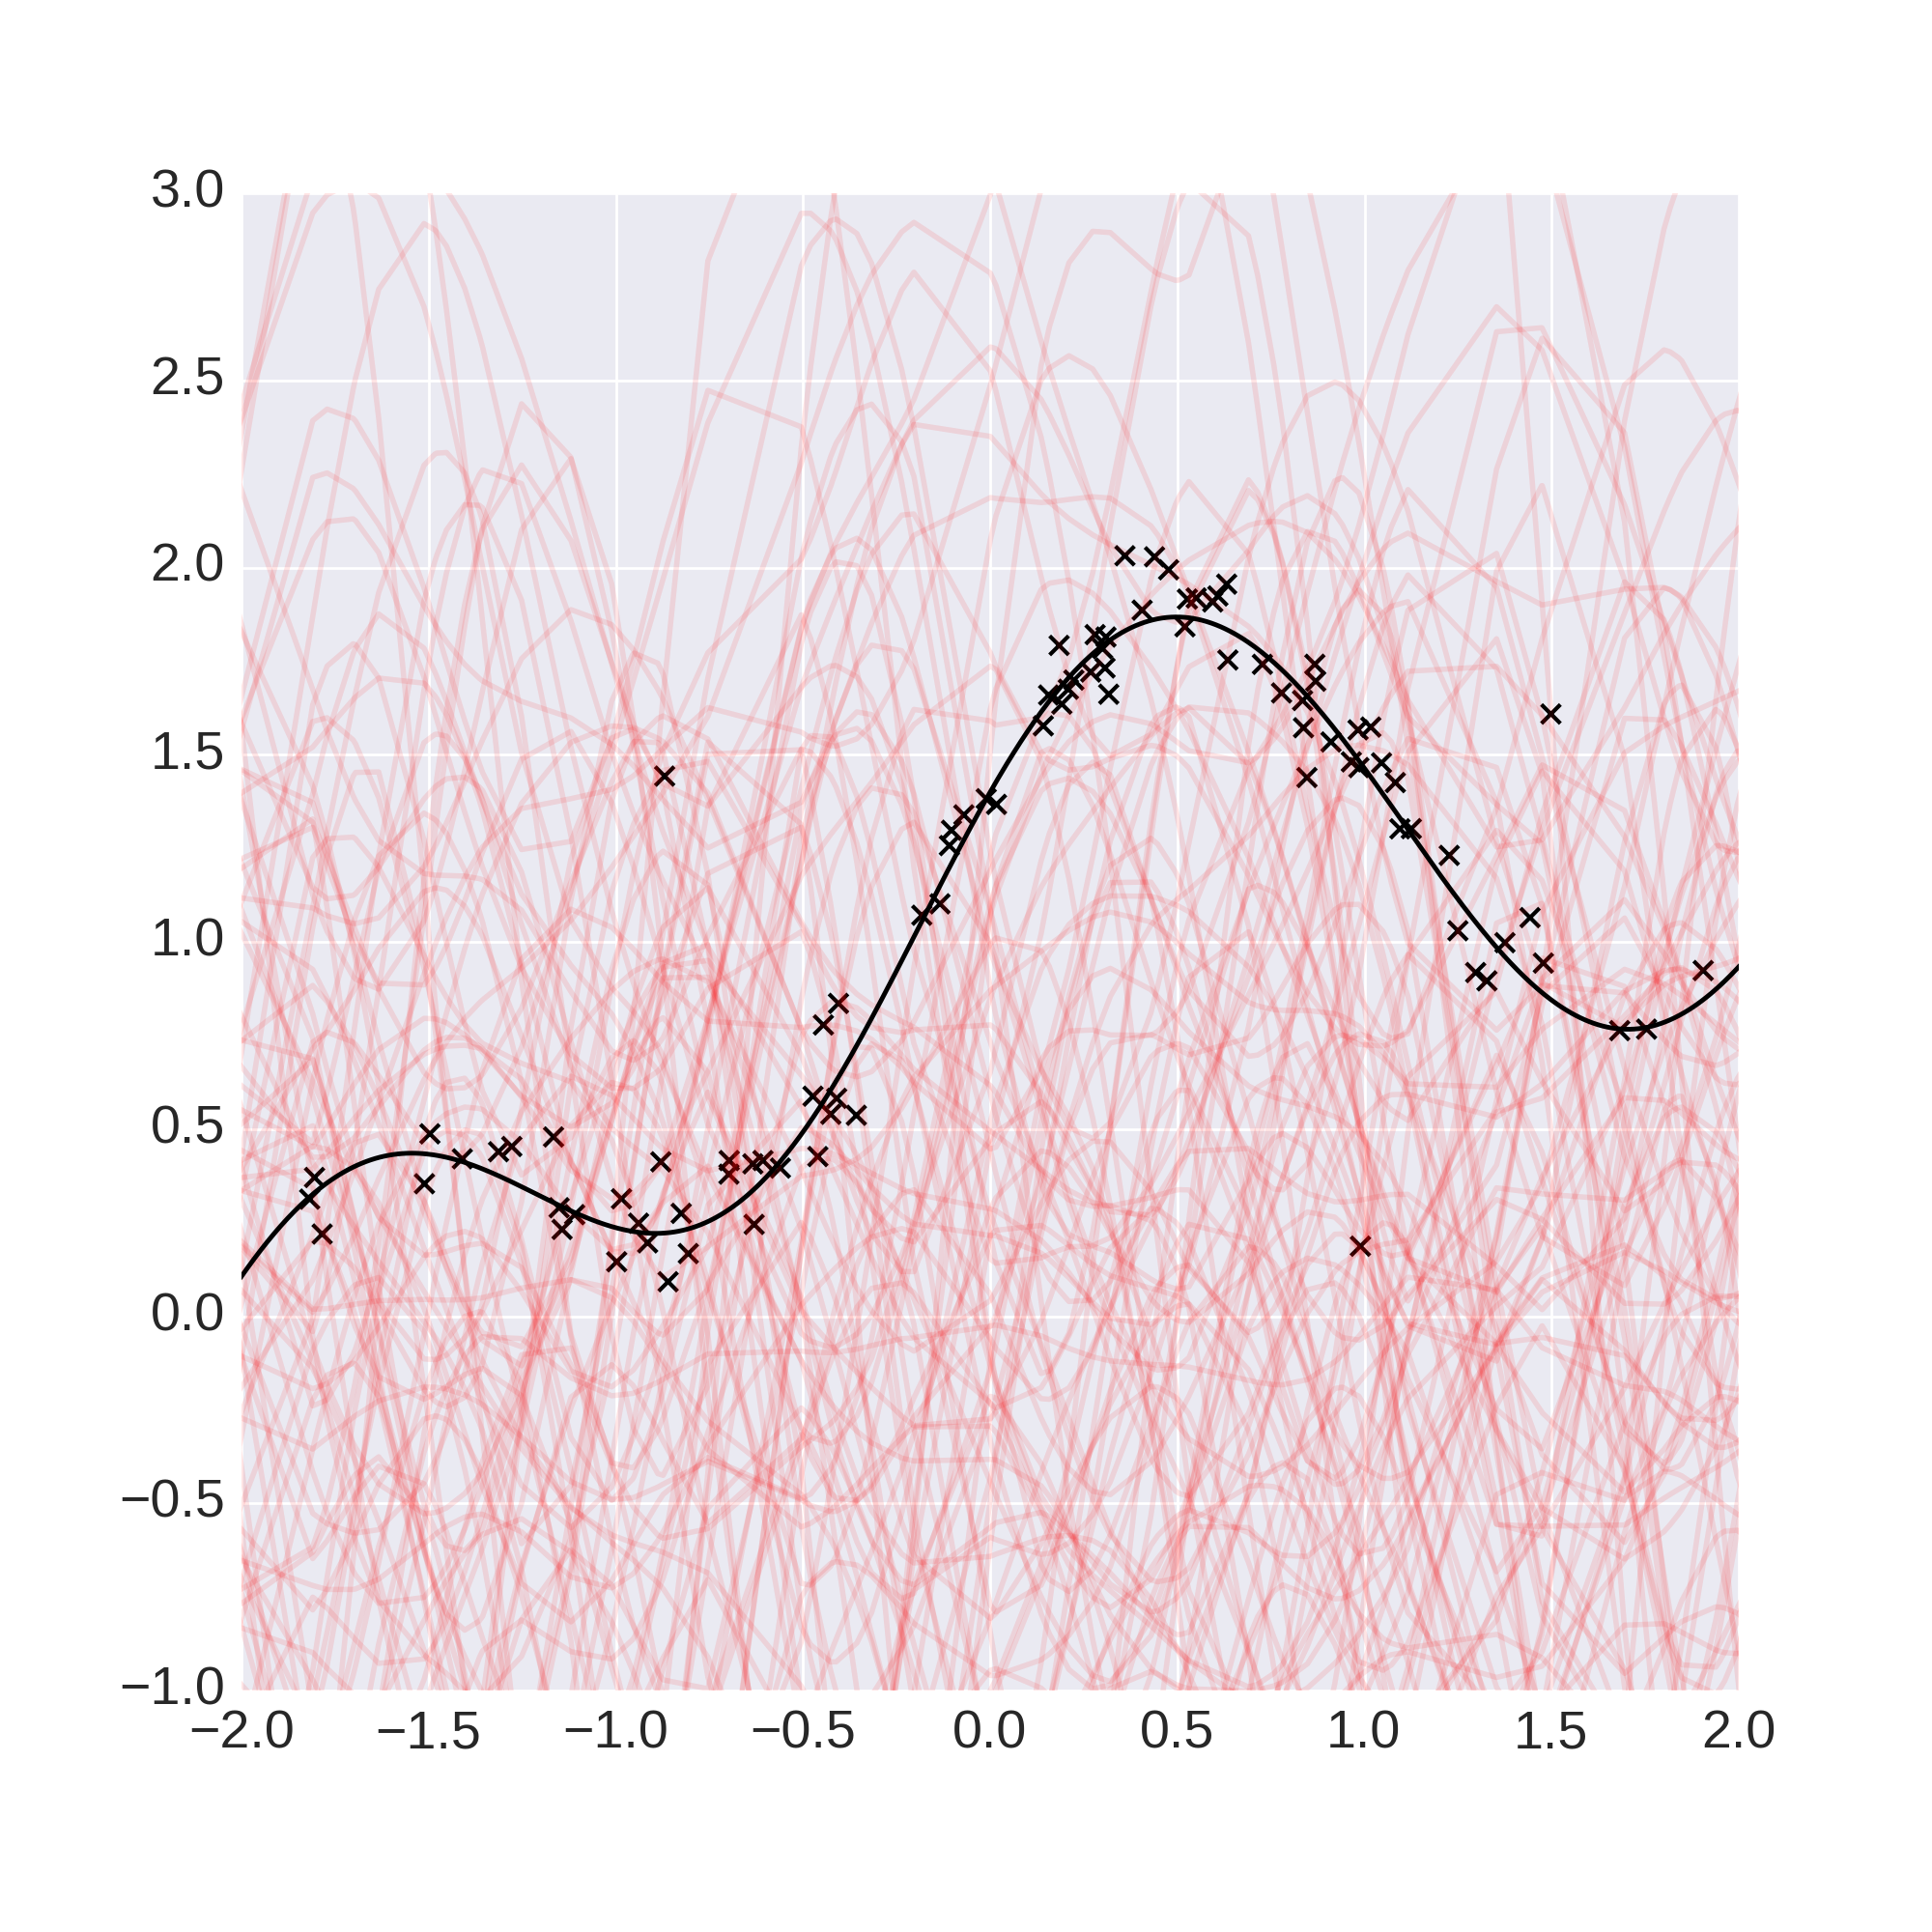
\includegraphics[height=4.5cm]{figs/neal_se_1a.png}
                \caption{Prior}
                \label{fig:NealBO}
        \end{subfigure}%
        ~ %add desired spacing between images, e. g. ~, \quad, \qquad, \hfill etc.
          %(or a blank line to force the subfigure onto a new line)
        \begin{subfigure}[b]{0.3\textwidth} \centering
                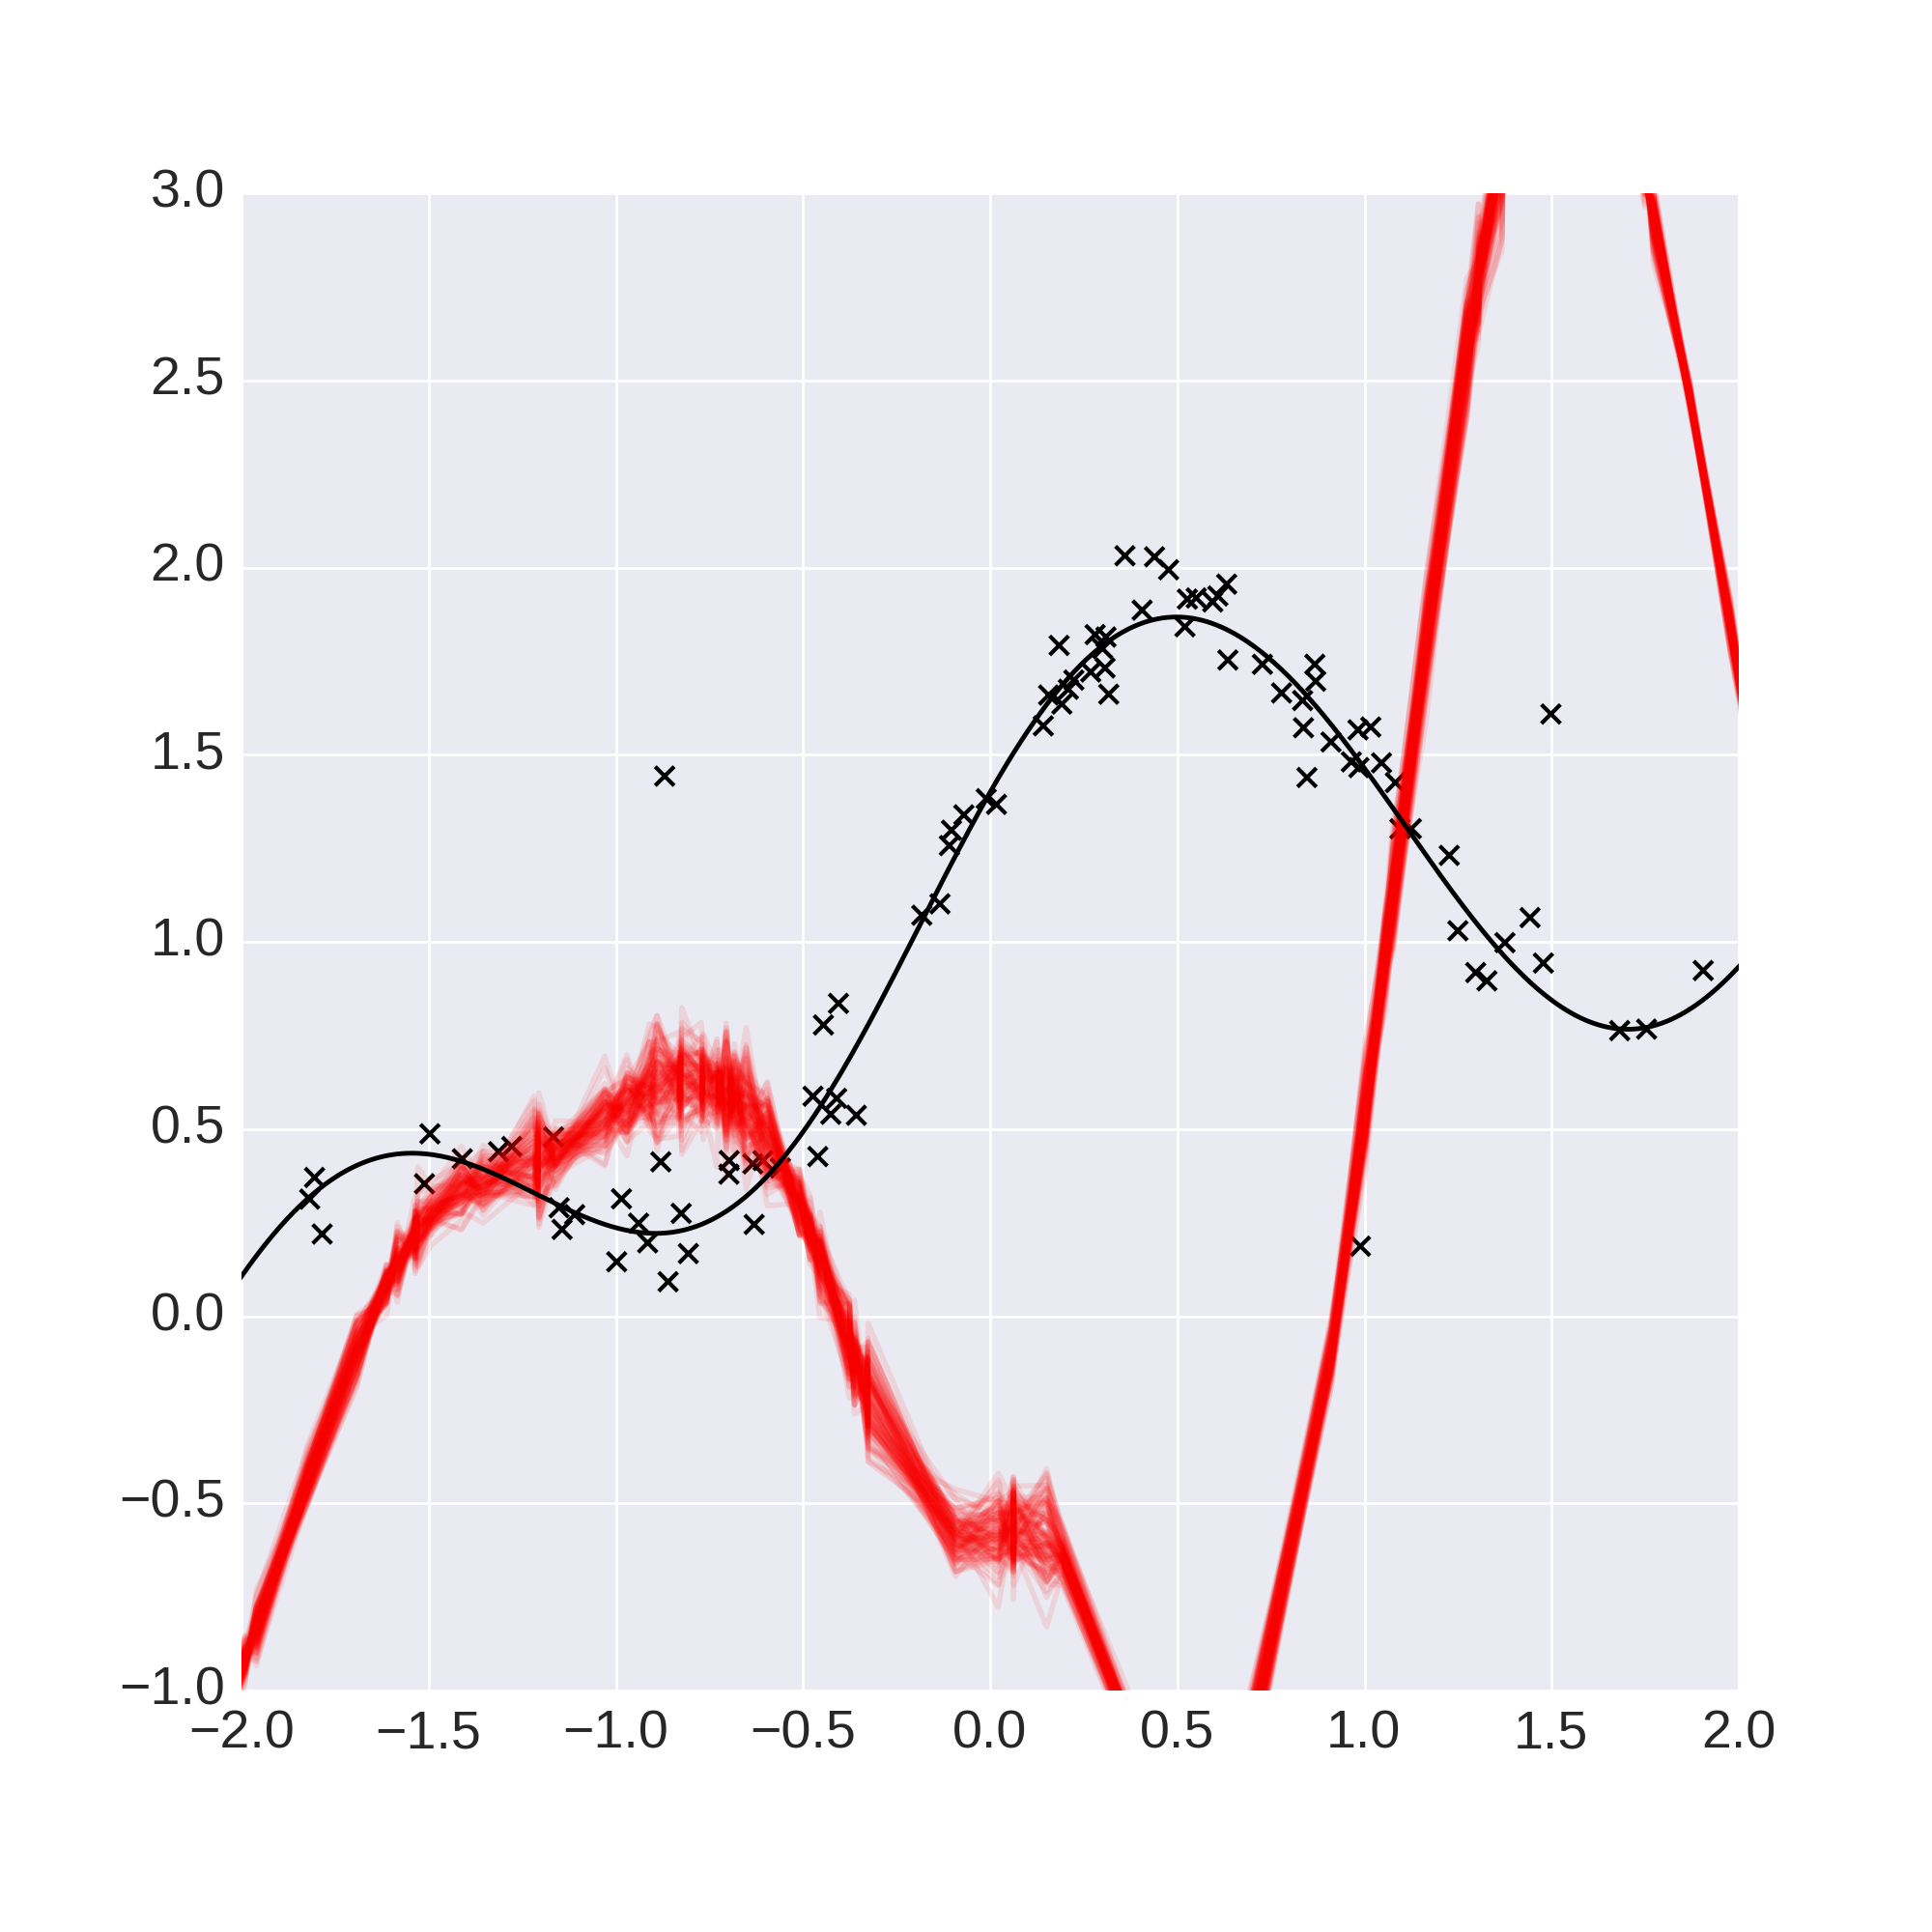
\includegraphics[height=4.5cm]{figs/neal_se_2a.png}
                \caption{Observed}
                \label{fig:NealAO))}
        \end{subfigure}
        ~ %add desired spacing between images, e. g. ~, \quad, \qquad, \hfill etc.
          %(or a blank line to force the subfigure onto a new line)
        \begin{subfigure}[b]{0.3\textwidth} \centering
                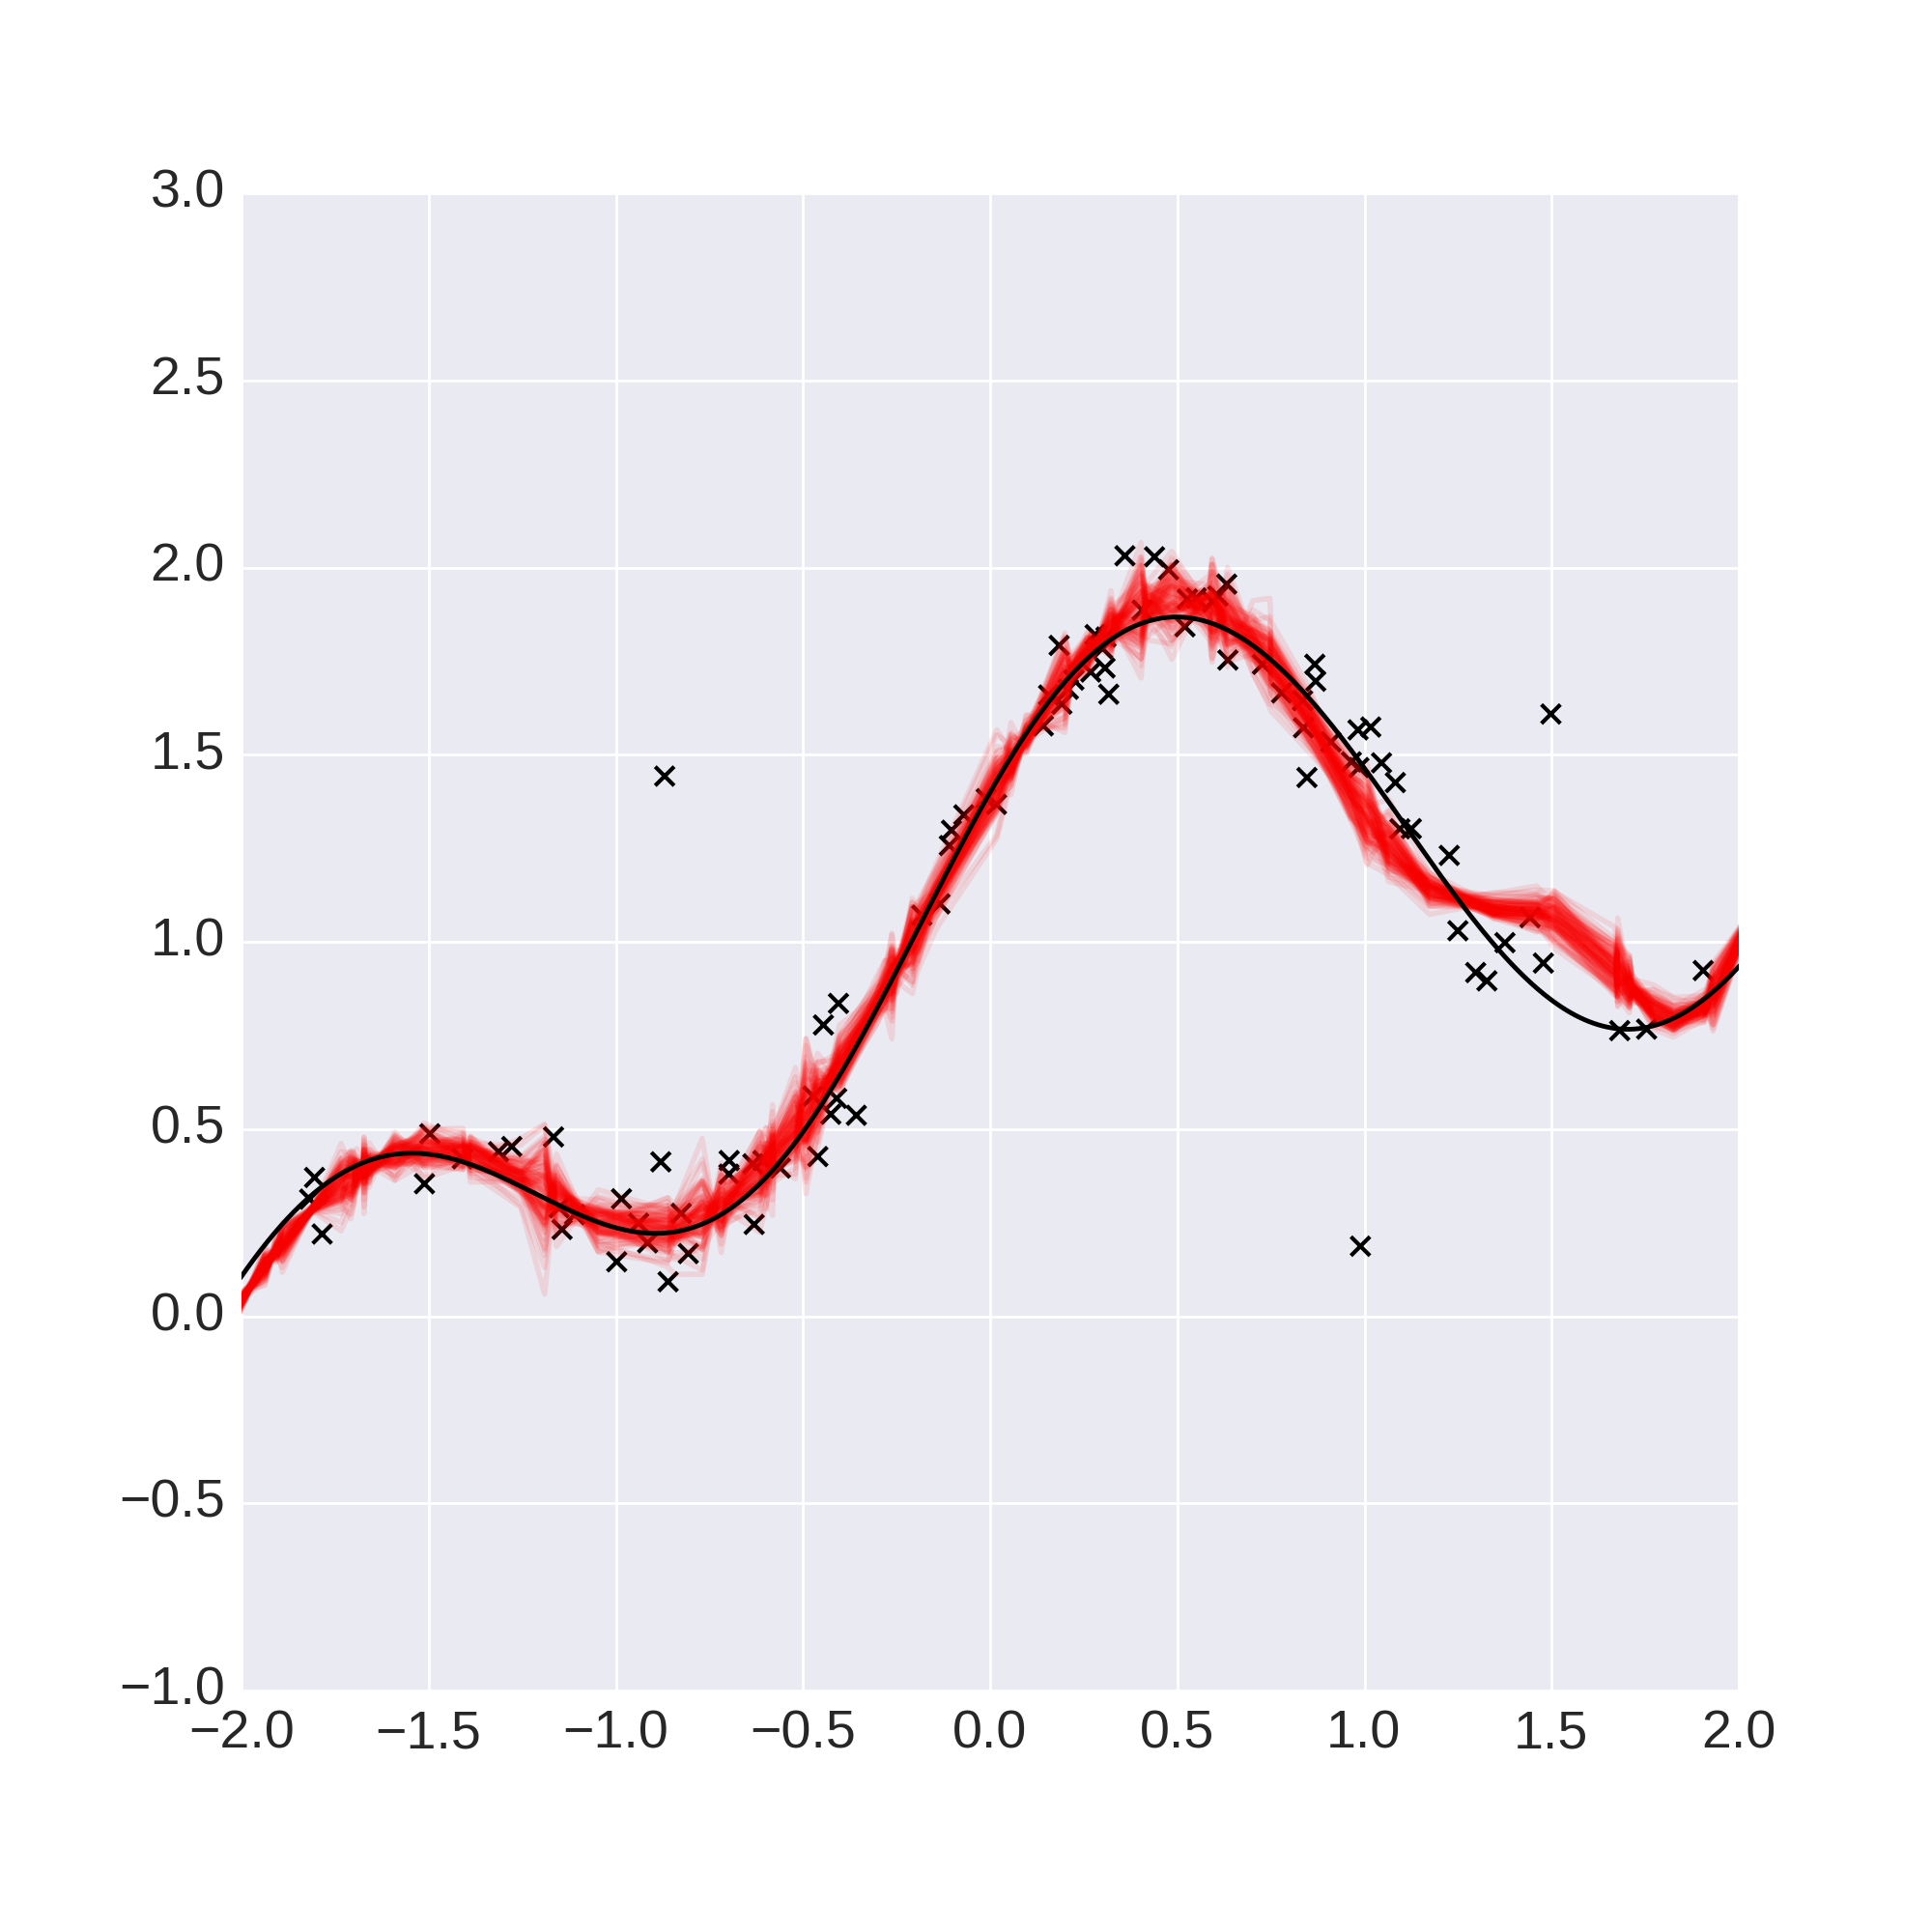
\includegraphics[height=4.5cm]{figs/neal_se_3a.png}
                \caption{Inferred}
                \label{fig:NealAI}
        \end{subfigure}
        \caption{Running a Venture GP on Neal's example for MCMC showing the prior, after having observed the data and after performing inference on the hyper-parameters. Note how the GP is choosing outliers to smooth instead of essential data. }\label{fig:neal}
\end{figure}


\subsection{Structure Learning}
Many equivalent covariance structures can be sampled due to covariance function algebra and equivalent representations with different parameterization~\citep{lloyd2014automatic}. Certain covariance functions can differ in terms of the hyper-parameterization but can be absorbed into a single covariance function with a different parameterization. To inspect the posterior of these equivalent structures we convert each kernel expression into a sum of products and subsequently simplify expressions using the following grammar:
\begin{minipage}{\linewidth}

\begin{lstlisting}[frame=single,label=alg:simplify,caption=Grammar to simplify expressions,mathescape]
SE $\times$ SE                  $\rightarrow$ SE 
{SE,PER,C,WN} $\times$ WN       $\rightarrow$ WN
LIN $+$ LIN                $\rightarrow$ LIN
{SE,PER,C,WN,LIN} $\times$ C    $\rightarrow$  {SE,PER,C,WN,LIN} 
\end{lstlisting}

\end{minipage}

For reproducing results from the Automated Statistician Project in a Bayesian fashion we first define a prior on the hypothesis space. Note that, as in the implementation of the Automated Statistician, we upper-bound the complexity of the space of covariance functions we want to explore. We also put vague priors on hyper-parameters.


\begin{minipage}{\linewidth}

\begin{lstlisting}[frame=single,label=alg:structureVent,caption=Venture Code for Bayesian GP Structure Learning,mathescape]
[ASSUME S (array K$_1$,K$_2$,$\cdots$,K$_n$)] // (defined as above)
[ASSUME p$_n$ (uniform_structure n)]
[ASSUME S (array K$_1$,K$_2$,$\cdots$,K$_n$)]
[ASSUME K$^*$ (grammar S p$_n$)]
[ASSUME GP (make-gp 0 K$^*$ ]

[OBSERVE GP D]

[INFER  (REPEAT 3000 (DO 
			(MH 10 p$_n$ one 1) 
			(MH 10 K$^*$ one 1) 
			(MH 10 {hyper-parameters} one 10)) ]


\end{lstlisting}

\end{minipage}

We defined a set of covariance structures so that we could reproduce results for covariance function structure learning as in the Automated Statistician. Our results are very similar to what has been reported by previous work (~\citealp*{duvenaud2013structure}; see Fig. \ref{fig:structure}).
\begin{figure}[p]

\centering
    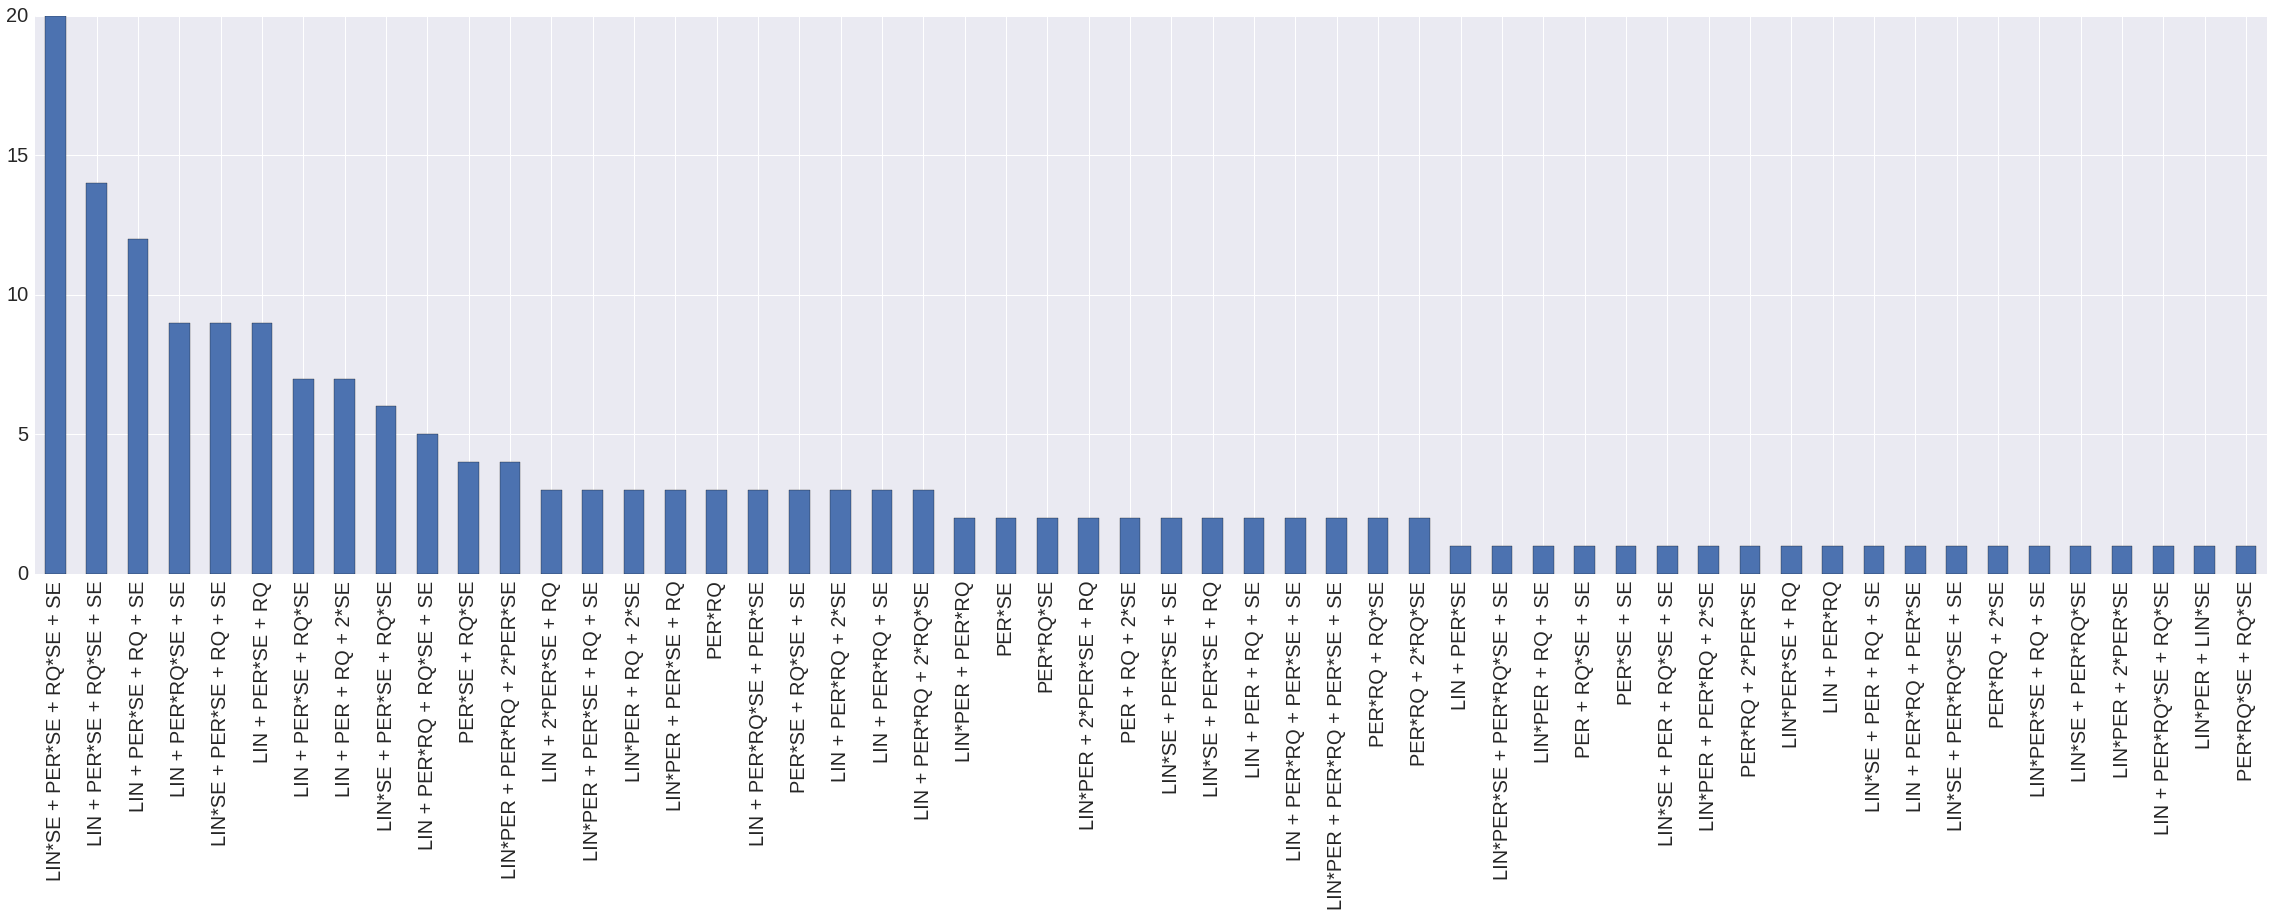
\includegraphics[width=\textwidth]{figs/prelimCO2structure.png}
    \caption{Preliminary results from the cross-validation on the CO2 data. Note that \citet{duvenaud2013structure} report LIN $\times$ SE $+$ PER $\times$ SE $+$ RQ $\times$ SE. We have run a leave one out cross-validation on this data set. Above we see the preliminary results on 181 validations (of a total of 545 $\times$ 2 runs).}\label{fig:structure}
\end{figure}

\begin{figure}
        \centering
        \begin{subfigure}[b]{\textwidth} \centering
                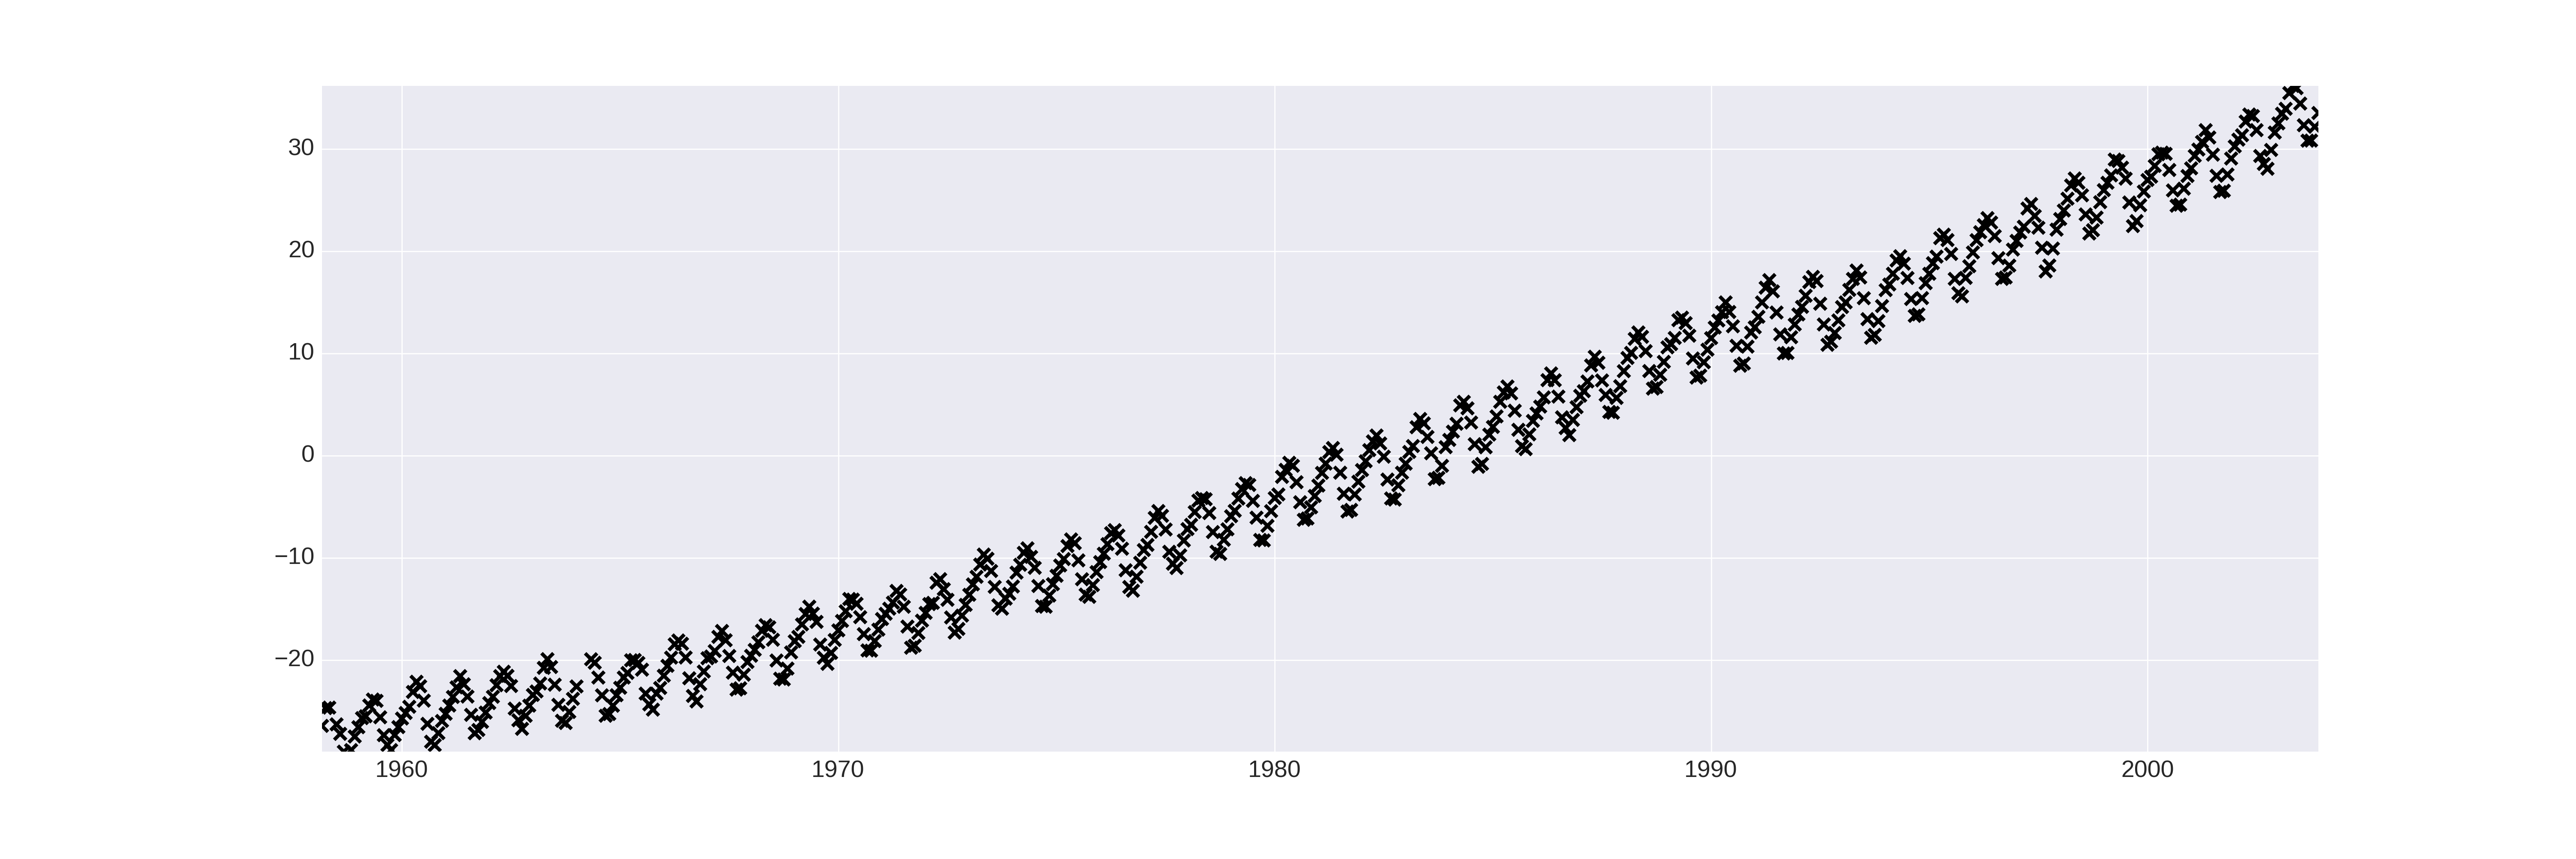
\includegraphics[height=3cm]{figs/airline_sexper_1a.png}
                \caption{Prior, before having seen any data.}
                \label{fig:airlineBO}
        \end{subfigure}%
        ~ %add desired spacing between images, e. g. ~, \quad, \qquad, \hfill etc.
          %(or a blank line to force the subfigure onto a new line)
          
        \begin{subfigure}[b]{\textwidth} \centering
                \includegraphics[height=3cm]{figs/airline_sexper_2a.png}
                \caption{After having seen any data but before inference}
                \label{fig:AirlineA))}
        \end{subfigure}
        ~ %add desired spacing between images, e. g. ~, \quad, \qquad, \hfill etc.
          %(or a blank line to force the subfigure onto a new line)
          
        \begin{subfigure}[b]{\textwidth} \centering
                \includegraphics[height=3cm]{figs/airline_sexper_3a.png}
                \caption{After 1000 MH steps.}
                \label{fig:airlineAI}
        \end{subfigure}
        \caption{Running a Venuter GP with covariance structure PER x SE on the airline data}\label{fig:airline}
\end{figure}

\subsection{Log-Likelihood}

%\begin{tcolorbox}
%       ripl.assume('l',"(tag (quote parameter) 0 (log (uniformcontinuous 0.01 8 )))")
%        ripl.assume('p',"(tag (quote parameter) 1 (log (uniform_continuous 0.1 8 )))")
%        ripl.assume('sf',"(tag (quote parameter) 2 (log (uniform_continuous 0.01 8 )))")
%        ripl.assume('gp',"""(tag (quote model) 0
                       %         (make_gp_part_der zero
                        %            (apply_function make_per l p sf )))""")

%\end{tcolorbox}
%\begin{figure}[p]
%\centering
%    % This file was created by matplotlib v0.1.0.
% Copyright (c) 2010--2014, Nico Schlömer <nico.schloemer@gmail.com>
% All rights reserved.
% 
% The lastest updates can be retrieved from
% 
% https://github.com/nschloe/matplotlib2tikz
% 
% where you can also submit bug reports and leavecomments.
% 
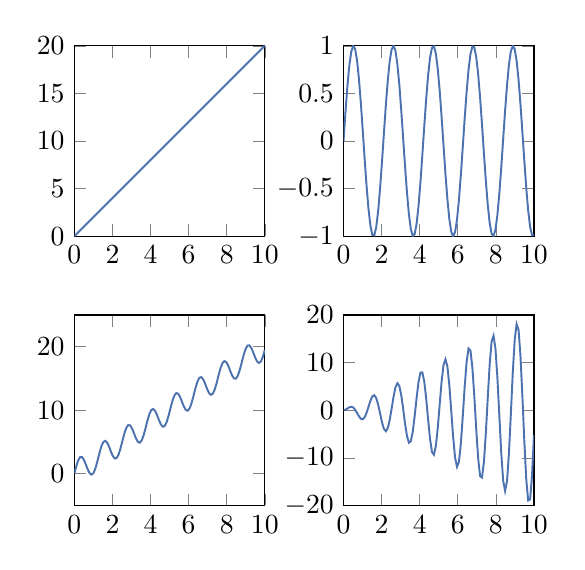
\begin{tikzpicture}

\definecolor{color0}{rgb}{0.298039215686275,0.447058823529412,0.690196078431373}

\begin{groupplot}[group style={group size=2 by 2}]
\nextgroupplot[
xmin=0, xmax=10,
ymin=0, ymax=20,
width=4cm,
height=4cm
]
\addplot [line width=0.7000000000000001pt, color0]
coordinates {
(0,0)
(0.101010101010101,0.202020202020202)
(0.202020202020202,0.404040404040404)
(0.303030303030303,0.606060606060606)
(0.404040404040404,0.808080808080808)
(0.505050505050505,1.01010101010101)
(0.606060606060606,1.21212121212121)
(0.707070707070707,1.41414141414141)
(0.808080808080808,1.61616161616162)
(0.909090909090909,1.81818181818182)
(1.01010101010101,2.02020202020202)
(1.11111111111111,2.22222222222222)
(1.21212121212121,2.42424242424242)
(1.31313131313131,2.62626262626263)
(1.41414141414141,2.82828282828283)
(1.51515151515152,3.03030303030303)
(1.61616161616162,3.23232323232323)
(1.71717171717172,3.43434343434343)
(1.81818181818182,3.63636363636364)
(1.91919191919192,3.83838383838384)
(2.02020202020202,4.04040404040404)
(2.12121212121212,4.24242424242424)
(2.22222222222222,4.44444444444444)
(2.32323232323232,4.64646464646465)
(2.42424242424242,4.84848484848485)
(2.52525252525253,5.05050505050505)
(2.62626262626263,5.25252525252525)
(2.72727272727273,5.45454545454545)
(2.82828282828283,5.65656565656566)
(2.92929292929293,5.85858585858586)
(3.03030303030303,6.06060606060606)
(3.13131313131313,6.26262626262626)
(3.23232323232323,6.46464646464646)
(3.33333333333333,6.66666666666667)
(3.43434343434343,6.86868686868687)
(3.53535353535354,7.07070707070707)
(3.63636363636364,7.27272727272727)
(3.73737373737374,7.47474747474747)
(3.83838383838384,7.67676767676768)
(3.93939393939394,7.87878787878788)
(4.04040404040404,8.08080808080808)
(4.14141414141414,8.28282828282828)
(4.24242424242424,8.48484848484848)
(4.34343434343434,8.68686868686869)
(4.44444444444444,8.88888888888889)
(4.54545454545454,9.09090909090909)
(4.64646464646465,9.29292929292929)
(4.74747474747475,9.49494949494949)
(4.84848484848485,9.6969696969697)
(4.94949494949495,9.8989898989899)
(5.05050505050505,10.1010101010101)
(5.15151515151515,10.3030303030303)
(5.25252525252525,10.5050505050505)
(5.35353535353535,10.7070707070707)
(5.45454545454545,10.9090909090909)
(5.55555555555556,11.1111111111111)
(5.65656565656566,11.3131313131313)
(5.75757575757576,11.5151515151515)
(5.85858585858586,11.7171717171717)
(5.95959595959596,11.9191919191919)
(6.06060606060606,12.1212121212121)
(6.16161616161616,12.3232323232323)
(6.26262626262626,12.5252525252525)
(6.36363636363636,12.7272727272727)
(6.46464646464646,12.9292929292929)
(6.56565656565657,13.1313131313131)
(6.66666666666667,13.3333333333333)
(6.76767676767677,13.5353535353535)
(6.86868686868687,13.7373737373737)
(6.96969696969697,13.9393939393939)
(7.07070707070707,14.1414141414141)
(7.17171717171717,14.3434343434343)
(7.27272727272727,14.5454545454545)
(7.37373737373737,14.7474747474747)
(7.47474747474747,14.9494949494949)
(7.57575757575758,15.1515151515152)
(7.67676767676768,15.3535353535354)
(7.77777777777778,15.5555555555556)
(7.87878787878788,15.7575757575758)
(7.97979797979798,15.959595959596)
(8.08080808080808,16.1616161616162)
(8.18181818181818,16.3636363636364)
(8.28282828282828,16.5656565656566)
(8.38383838383838,16.7676767676768)
(8.48484848484848,16.969696969697)
(8.58585858585859,17.1717171717172)
(8.68686868686869,17.3737373737374)
(8.78787878787879,17.5757575757576)
(8.88888888888889,17.7777777777778)
(8.98989898989899,17.979797979798)
(9.09090909090909,18.1818181818182)
(9.19191919191919,18.3838383838384)
(9.29292929292929,18.5858585858586)
(9.39393939393939,18.7878787878788)
(9.49494949494949,18.989898989899)
(9.5959595959596,19.1919191919192)
(9.6969696969697,19.3939393939394)
(9.7979797979798,19.5959595959596)
(9.8989898989899,19.7979797979798)
(10,20)

};
\path [draw=white!15.0!black, fill opacity=0] (axis cs:13,20)--(axis cs:13,20);

\path [draw=white!15.0!black, fill opacity=0] (axis cs:10,13)--(axis cs:10,13);

\path [draw=white!15.0!black, fill opacity=0] (axis cs:13,0)--(axis cs:13,0);

\path [draw=white!15.0!black, fill opacity=0] (axis cs:0,13)--(axis cs:0,13);

\nextgroupplot[
xmin=0, xmax=10,
ymin=-1, ymax=1,
width=4cm,
height=4cm
]
\addplot [line width=0.7000000000000001pt, color0]
coordinates {
(-3.5527136788005e-15,0)
(0.101010101010097,0.298413804447641)
(0.202020202020198,0.569634106908966)
(0.303030303030299,0.788945462844257)
(0.4040404040404,0.936362725104285)
(0.505050505050502,0.998452226900389)
(0.606060606060603,0.969555949182324)
(0.707070707070704,0.852307117939675)
(0.808080808080805,0.657390246682775)
(0.909090909090906,0.402567490669497)
(1.01010101010101,0.11106003812413)
(1.11111111111111,-0.190567962875485)
(1.21212121212121,-0.47483011082224)
(1.31313131313131,-0.71582249922919)
(1.41414141414141,-0.89158425733514)
(1.51515151515151,-0.98609877449093)
(1.61616161616161,-0.990753243005677)
(1.71717171717171,-0.905123515950137)
(1.81818181818181,-0.737012758318913)
(1.91919191919192,-0.501740369393911)
(2.02020202020202,-0.220745974555063)
(2.12121212121212,0.0803642996702817)
(2.22222222222222,0.37415123057122)
(2.32323232323232,0.633842948448905)
(2.42424242424242,0.835774572052259)
(2.52525252525252,0.961544714026824)
(2.62626262626262,0.999692340886112)
(2.72727272727272,0.946741180583354)
(2.82828282828282,0.807516504139563)
(2.92929292929293,0.594705414024498)
(3.03030303030303,0.3277007088135)
(3.13131313131313,0.0308336790611428)
(3.23232323232323,-0.268843125910384)
(3.33333333333333,-0.54402111088937)
(3.43434343434343,-0.769624180301191)
(3.53535353535353,-0.925093843135269)
(3.63636363636363,-0.996262642919822)
(3.73737373737373,-0.976645193022395)
(3.83838383838383,-0.868029169330635)
(3.93939393939394,-0.680312405027813)
(4.04040404040404,-0.430600932498663)
(4.14141414141414,-0.141650164941304)
(4.24242424242424,0.160208732147209)
(4.34343434343434,0.447468316432701)
(4.44444444444444,0.693951534577056)
(4.54545454545454,0.877197153948597)
(4.64646464646464,0.980506583396065)
(4.74747474747474,0.994465562811467)
(4.84848484848485,0.917802054746127)
(4.94949494949495,0.757502161142318)
(5.05050505050505,0.528173502056996)
(5.15151515151515,0.25071406965208)
(5.25252525252525,-0.0495921394416738)
(5.35353535353535,-0.345379174414414)
(5.45454545454545,-0.609692902437243)
(5.55555555555555,-0.818447253157943)
(5.65656565656565,-0.952619105774571)
(5.75757575757575,-0.999981805600717)
(5.85858585858585,-0.956219340264959)
(5.95959595959596,-0.825319644206981)
(6.06060606060606,-0.61921119088112)
(6.16161616161616,-0.356675988865319)
(6.26262626262626,-0.0616380370868764)
(6.36363636363636,0.239016793197097)
(6.46464646464646,0.517890782435197)
(6.56565656565656,0.749571029926278)
(6.66666666666666,0.912945250727628)
(6.76767676767676,0.993125671111422)
(6.86868686868686,0.982805704088478)
(6.96969696969697,0.882925775468708)
(7.07070707070707,0.702587625844653)
(7.17171717171717,0.458224897886049)
(7.27272727272727,0.172105590690409)
(7.37373737373737,-0.129697152232876)
(7.47474747474747,-0.419681005700317)
(7.57575757575757,-0.671420662377814)
(7.67676767676767,-0.861975887089034)
(7.77777777777777,-0.973981987569556)
(7.87878787878788,-0.997232203708085)
(7.97979797979798,-0.92960781717014)
(8.08080808080808,-0.777271223469046)
(8.18181818181818,-0.554104372439755)
(8.28282828282828,-0.280443750251132)
(8.38383838383838,0.0187728199728824)
(8.48484848484848,0.316278682751012)
(8.58585858585858,0.584963073936907)
(8.68686868686868,0.800341638529193)
(8.78787878787878,0.942787612159873)
(8.88888888888889,0.999320345780098)
(8.98989898989899,0.964788190970519)
(9.09090909090909,0.842337953295793)
(9.19191919191919,0.643128133910366)
(9.29292929292929,0.385312090797061)
(9.39393939393939,0.0923837809243858)
(9.49494949494949,-0.208963169415405)
(9.59595959595959,-0.491267969968986)
(9.69696969696969,-0.728805081099179)
(9.79797979797979,-0.899928500486141)
(9.8989898989899,-0.989044294552925)
(10,-0.988031624092862)

};
\path [draw=white!15.0!black, fill opacity=0] (axis cs:13,1)--(axis cs:13,1);

\path [draw=white!15.0!black, fill opacity=0] (axis cs:10,13)--(axis cs:10,13);

\path [draw=white!15.0!black, fill opacity=0] (axis cs:13,-1)--(axis cs:13,-1);

\path [draw=white!15.0!black, fill opacity=0] (axis cs:-3.5527136788005e-15,13)--(axis cs:-3.5527136788005e-15,13);

\nextgroupplot[
xmin=0, xmax=10,
ymin=-5, ymax=25,
width=4cm,
height=4cm
]
\addplot [line width=0.7000000000000001pt, color0]
coordinates {
(0,0)
(0.101010101010101,1.16972348289607)
(0.202020202020202,2.09781153124637)
(0.303030303030303,2.60296505986138)
(0.404040404040404,2.60949170048672)
(0.505050505050505,2.16620618031416)
(0.606060606060606,1.43424128836947)
(0.707070707070707,0.646813030529189)
(0.808080808080808,0.0509866108532118)
(0.909090909090909,-0.154015730800041)
(1.01010101010101,0.133439503310022)
(1.11111111111111,0.892019192264577)
(1.21212121212121,1.9827504751323)
(1.31313131313131,3.18372226361774)
(1.41414141414141,4.24549642368126)
(1.51515151515152,4.95339245835668)
(1.61616161616162,5.1810932112743)
(1.71717171717172,4.92218625085713)
(1.81818181818182,4.29176505399064)
(1.91919191919192,3.49769017372765)
(2.02020202020202,2.78868647523401)
(2.12121212121212,2.3922365561537)
(2.22222222222222,2.45777835953462)
(2.32323232323232,3.01939053098336)
(2.42424242424242,3.98728298348752)
(2.52525252525253,5.17021747521253)
(2.62626262626263,6.32325978372769)
(2.72727272727273,7.20893976244265)
(2.82828282828283,7.65654761788272)
(2.92929292929293,7.60476013194383)
(3.03030303030303,7.11695306472005)
(3.13131313131313,6.36537623209961)
(3.23232323232323,5.58814274003209)
(3.33333333333333,5.02977216035078)
(3.43434343434343,4.88013401255833)
(3.53535353535354,5.22703735946139)
(3.63636363636364,6.03430489096503)
(3.73737373737374,7.15080639561124)
(3.83838383838384,8.34819596271544)
(3.93939393939394,9.37792993864043)
(4.04040404040404,10.0333282579265)
(4.14141414141414,10.2011824396848)
(4.24242424242424,9.89002373653779)
(4.34343434343434,9.22799288149768)
(4.44444444444444,8.43084335682357)
(4.54545454545454,7.74806776615346)
(4.64646464646465,7.40059955063213)
(4.74747474747475,7.52564592570927)
(4.84848484848485,8.14242725003161)
(4.94949494949495,9.14737770337224)
(5.05050505050505,10.3400056639479)
(5.15151515151515,11.4729564509041)
(5.25252525252525,12.313776769033)
(5.35353535353535,12.702958278646)
(5.45454545454545,12.5937668156825)
(5.55555555555556,12.0639119088691)
(5.65656565656566,11.2961427163943)
(5.75757575757576,10.5326155752135)
(5.85858585858586,10.0144275824015)
(5.95959595959596,9.92141466862103)
(6.06060606060606,10.3272465801163)
(6.16161616161616,11.1810315487621)
(6.26262626262626,12.3200239626361)
(6.36363636363636,13.5102619327555)
(6.46464646464646,14.5049875586983)
(6.56565656565657,15.1062623572933)
(6.66666666666667,15.2143924865909)
(6.76767676767677,14.8528222905033)
(6.86868686868687,14.1622802479392)
(6.96969696969697,13.3656390824819)
(7.07070707070707,12.7122644605122)
(7.17171717171717,12.4157484035596)
(7.27272727272727,12.6005753770117)
(7.37373737373737,13.2710385287151)
(7.47474747474747,14.3101676902889)
(7.57575757575758,15.5089368191422)
(7.67676767676768,16.6184577851754)
(7.77777777777778,17.4121277176568)
(7.87878787878788,17.7422117245549)
(7.97979797979798,17.5767322836758)
(8.08080808080808,17.0074540274871)
(8.18181818181818,16.2269701214737)
(8.28282828282828,15.4806117655801)
(8.38383838383838,15.0051890125201)
(8.48484848484848,14.969859315891)
(8.58585858585859,15.4338889270665)
(8.68686868686869,16.3318541168028)
(8.78787878787879,17.4899774753814)
(8.88888888888889,18.6695201184033)
(8.98989898989899,19.6263947677971)
(9.09090909090909,20.1721143263146)
(9.19191919191919,20.2208570911657)
(9.29292929292929,19.8108964265813)
(9.39393939393939,19.0950439077188)
(9.49494949494949,18.3024922821398)
(9.5959595959596,17.6815860584331)
(9.6969696969697,17.4378099015879)
(9.7979797979798,17.6824791280055)
(9.8989898989899,18.4049442795857)
(10,19.4752502925921)

};
\path [draw=white!15.0!black, fill opacity=0] (axis cs:13,25)--(axis cs:13,25);

\path [draw=white!15.0!black, fill opacity=0] (axis cs:10,13)--(axis cs:10,13);

\path [draw=white!15.0!black, fill opacity=0] (axis cs:13,-5)--(axis cs:13,-5);

\path [draw=white!15.0!black, fill opacity=0] (axis cs:0,13)--(axis cs:0,13);

\nextgroupplot[
xmin=0, xmax=10,
ymin=-20, ymax=20,
width=4cm,
height=4cm
]
\addplot [line width=0.7000000000000001pt, color0]
coordinates {
(-3.5527136788005e-15,0)
(0.101010101010097,0.0977478061490777)
(0.202020202020198,0.342175985294135)
(0.303030303030299,0.605122561757812)
(0.4040404040404,0.727842784810469)
(0.505050505050502,0.583891500107649)
(0.606060606060603,0.134618228029248)
(0.707070707070704,-0.542555422756118)
(0.808080808080805,-1.2647878830775)
(0.909090909090906,-1.79290686271078)
(1.01010101010101,-1.90582072413333)
(1.11111111111111,-1.47800336661961)
(1.21212121212121,-0.535141756497123)
(1.31313131313131,0.732017705617827)
(1.41414141414141,2.00414043793718)
(1.51515151515151,2.91377186068734)
(1.61616161616161,3.1495272387088)
(1.71717171717171,2.55488160411442)
(1.81818181818181,1.19163894114)
(1.91919191919192,-0.653856528128047)
(2.02020202020202,-2.52872235387886)
(2.12121212121212,-3.92464054663447)
(2.22222222222222,-4.41481352202183)
(2.32323232323232,-3.78007117738076)
(2.42424242424242,-2.08776209696322)
(2.52525252525252,0.302304102796675)
(2.62626262626262,2.81203008194579)
(2.72727272727272,4.78471174881053)
(2.82828282828282,5.65651463806847)
(2.92929292929293,5.11505595226072)
(3.03030303030303,3.20105152761815)
(3.13131313131313,0.32174232865393)
(3.23232323232323,-2.83314335228889)
(3.33333333333333,-5.45631502105297)
(3.43434343434343,-6.82937344528993)
(3.53535353535353,-6.51802423167664)
(3.63636363636363,-4.50335411549905)
(3.73737373737373,-1.21068888162028)
(3.83838383838383,2.57719948141566)
(3.93939393939394,5.90571114487371)
(4.04040404040404,7.88897041259968)
(4.14141414141414,7.94469903344625)
(4.24242424242424,5.96134955262129)
(4.34343434343434,2.35033741101484)
(4.44444444444444,-2.03575792029029)
(4.54545454545454,-6.10382420343467)
(4.64646464646464,-8.79264324703732)
(4.74747474747474,-9.34921896507985)
(4.84848484848485,-7.5371755003059)
(4.94949494949495,-3.72010076618844)
(5.05050505050505,1.20704829766579)
(5.15151515151515,6.02689227692571)
(5.25252525252525,9.50038037647393)
(5.35353535353535,10.6850546761101)
(5.45454545454545,9.18914130868138)
(5.55555555555555,5.29333776532232)
(5.65656565656565,-0.096097112855695)
(5.75757575757575,-5.65702510873381)
(5.85858585858585,-9.97567270875466)
(5.95959595959596,-11.905945230675)
(6.06060606060606,-10.8725184308835)
(6.16161616161616,-7.03780275178642)
(6.26262626262626,-1.28526978608287)
(6.36363636363636,4.98265858034507)
(6.46464646464646,10.186308715348)
(6.56565656565656,12.9668383523951)
(6.66666666666666,12.5403943550502)
(6.76767676767676,8.91620268636688)
(6.86868686868686,2.91854976954049)
(6.96969696969697,-3.99889748756882)
(7.07070707070707,-10.1050987538521)
(7.17171717171717,-13.8248183566775)
(7.27272727272727,-14.1445757704931)
(7.37373737373737,-10.8868529262077)
(7.47474747474747,-4.77880981628743)
(7.57575757575757,2.70773990626534)
(7.67676767676767,9.71051563683239)
(7.77777777777777,14.4400057052322)
(7.87878787878788,15.6365258004418)
(7.97979797979798,12.90442117195)
(8.08080808080808,6.83505346158356)
(8.18181818181818,-1.11817834496734)
(8.28282828282828,-8.98723975820886)
(8.38383838383838,-14.7764124927275)
(8.48484848484848,-16.9683194868385)
(8.58585858585858,-14.9207475550816)
(8.68686868686868,-9.05070304003775)
(8.78787878787878,-0.753825124517871)
(8.88888888888889,7.92659858333792)
(8.98989898989899,14.8027388012045)
(9.09090909090909,18.0936013136041)
(9.19191919191919,16.8857275117966)
(9.29292929292929,11.3841900349987)
(9.39393939393939,2.88549051970944)
(9.49494949494949,-6.52689197266276)
(9.59595959595959,-14.4930957253715)
(9.69696969696969,-18.9685284106814)
(9.79797979797979,-18.7482429688431)
(9.8989898989899,-13.7896445255172)
(10,-5.24749707407858)

};
\path [draw=white!15.0!black, fill opacity=0] (axis cs:13,20)--(axis cs:13,20);

\path [draw=white!15.0!black, fill opacity=0] (axis cs:10,13)--(axis cs:10,13);

\path [draw=white!15.0!black, fill opacity=0] (axis cs:13,-20)--(axis cs:13,-20);

\path [draw=white!15.0!black, fill opacity=0] (axis cs:-3.5527136788005e-15,13)--(axis cs:-3.5527136788005e-15,13);

\end{groupplot}

\end{tikzpicture}
%    \caption{We show how the log-Likelihood evolves over an MCMC chain for different test problems. We see how the correct %structures scores highest for each test problems while requiring few datapoint.}

%\end{figure}

\subsection{Residuals}
\bibliography{May2015}
\bibliographystyle{apalike}
\end{document}
